% Options for packages loaded elsewhere
\PassOptionsToPackage{unicode}{hyperref}
\PassOptionsToPackage{hyphens}{url}
%
\documentclass[
  12pt,
]{article}
\usepackage{amsmath,amssymb}
\usepackage{lmodern}
\usepackage{setspace}
\usepackage{ifxetex,ifluatex}
\ifnum 0\ifxetex 1\fi\ifluatex 1\fi=0 % if pdftex
  \usepackage[T1]{fontenc}
  \usepackage[utf8]{inputenc}
  \usepackage{textcomp} % provide euro and other symbols
\else % if luatex or xetex
  \usepackage{unicode-math}
  \defaultfontfeatures{Scale=MatchLowercase}
  \defaultfontfeatures[\rmfamily]{Ligatures=TeX,Scale=1}
\fi
% Use upquote if available, for straight quotes in verbatim environments
\IfFileExists{upquote.sty}{\usepackage{upquote}}{}
\IfFileExists{microtype.sty}{% use microtype if available
  \usepackage[]{microtype}
  \UseMicrotypeSet[protrusion]{basicmath} % disable protrusion for tt fonts
}{}
\makeatletter
\@ifundefined{KOMAClassName}{% if non-KOMA class
  \IfFileExists{parskip.sty}{%
    \usepackage{parskip}
  }{% else
    \setlength{\parindent}{0pt}
    \setlength{\parskip}{6pt plus 2pt minus 1pt}}
}{% if KOMA class
  \KOMAoptions{parskip=half}}
\makeatother
\usepackage{xcolor}
\IfFileExists{xurl.sty}{\usepackage{xurl}}{} % add URL line breaks if available
\IfFileExists{bookmark.sty}{\usepackage{bookmark}}{\usepackage{hyperref}}
\hypersetup{
  pdftitle={Standardized NEON organismal data for biodiversity research},
  pdfauthor={Daijiang Li1,2†‡, Sydne Record3†‡, Eric Sokol4,5†‡, Matthew E. Bitters6, Melissa Y. Chen6, Anny Y. Chung7, Matthew R. Helmus8, Ruvi Jaimes9, Lara Jansen10, Marta A. Jarzyna11,12, Michael G. Just13, Jalene M. LaMontagne14, Brett Melbourne6, Wynne Moss6, Kari Norman15, Stephanie Parker4, Natalie Robinson4, Bijan Seyednasrollah16, Colin Smith17, Sarah Spaulding5, Thilina Surasinghe18, Sarah Thomsen19, Phoebe Zarnetske20,21},
  hidelinks,
  pdfcreator={LaTeX via pandoc}}
\urlstyle{same} % disable monospaced font for URLs
\usepackage[margin=1in]{geometry}
\usepackage{color}
\usepackage{fancyvrb}
\newcommand{\VerbBar}{|}
\newcommand{\VERB}{\Verb[commandchars=\\\{\}]}
\DefineVerbatimEnvironment{Highlighting}{Verbatim}{commandchars=\\\{\}}
% Add ',fontsize=\small' for more characters per line
\usepackage{framed}
\definecolor{shadecolor}{RGB}{248,248,248}
\newenvironment{Shaded}{\begin{snugshade}}{\end{snugshade}}
\newcommand{\AlertTok}[1]{\textcolor[rgb]{0.94,0.16,0.16}{#1}}
\newcommand{\AnnotationTok}[1]{\textcolor[rgb]{0.56,0.35,0.01}{\textbf{\textit{#1}}}}
\newcommand{\AttributeTok}[1]{\textcolor[rgb]{0.77,0.63,0.00}{#1}}
\newcommand{\BaseNTok}[1]{\textcolor[rgb]{0.00,0.00,0.81}{#1}}
\newcommand{\BuiltInTok}[1]{#1}
\newcommand{\CharTok}[1]{\textcolor[rgb]{0.31,0.60,0.02}{#1}}
\newcommand{\CommentTok}[1]{\textcolor[rgb]{0.56,0.35,0.01}{\textit{#1}}}
\newcommand{\CommentVarTok}[1]{\textcolor[rgb]{0.56,0.35,0.01}{\textbf{\textit{#1}}}}
\newcommand{\ConstantTok}[1]{\textcolor[rgb]{0.00,0.00,0.00}{#1}}
\newcommand{\ControlFlowTok}[1]{\textcolor[rgb]{0.13,0.29,0.53}{\textbf{#1}}}
\newcommand{\DataTypeTok}[1]{\textcolor[rgb]{0.13,0.29,0.53}{#1}}
\newcommand{\DecValTok}[1]{\textcolor[rgb]{0.00,0.00,0.81}{#1}}
\newcommand{\DocumentationTok}[1]{\textcolor[rgb]{0.56,0.35,0.01}{\textbf{\textit{#1}}}}
\newcommand{\ErrorTok}[1]{\textcolor[rgb]{0.64,0.00,0.00}{\textbf{#1}}}
\newcommand{\ExtensionTok}[1]{#1}
\newcommand{\FloatTok}[1]{\textcolor[rgb]{0.00,0.00,0.81}{#1}}
\newcommand{\FunctionTok}[1]{\textcolor[rgb]{0.00,0.00,0.00}{#1}}
\newcommand{\ImportTok}[1]{#1}
\newcommand{\InformationTok}[1]{\textcolor[rgb]{0.56,0.35,0.01}{\textbf{\textit{#1}}}}
\newcommand{\KeywordTok}[1]{\textcolor[rgb]{0.13,0.29,0.53}{\textbf{#1}}}
\newcommand{\NormalTok}[1]{#1}
\newcommand{\OperatorTok}[1]{\textcolor[rgb]{0.81,0.36,0.00}{\textbf{#1}}}
\newcommand{\OtherTok}[1]{\textcolor[rgb]{0.56,0.35,0.01}{#1}}
\newcommand{\PreprocessorTok}[1]{\textcolor[rgb]{0.56,0.35,0.01}{\textit{#1}}}
\newcommand{\RegionMarkerTok}[1]{#1}
\newcommand{\SpecialCharTok}[1]{\textcolor[rgb]{0.00,0.00,0.00}{#1}}
\newcommand{\SpecialStringTok}[1]{\textcolor[rgb]{0.31,0.60,0.02}{#1}}
\newcommand{\StringTok}[1]{\textcolor[rgb]{0.31,0.60,0.02}{#1}}
\newcommand{\VariableTok}[1]{\textcolor[rgb]{0.00,0.00,0.00}{#1}}
\newcommand{\VerbatimStringTok}[1]{\textcolor[rgb]{0.31,0.60,0.02}{#1}}
\newcommand{\WarningTok}[1]{\textcolor[rgb]{0.56,0.35,0.01}{\textbf{\textit{#1}}}}
\usepackage{longtable,booktabs,array}
\usepackage{calc} % for calculating minipage widths
% Correct order of tables after \paragraph or \subparagraph
\usepackage{etoolbox}
\makeatletter
\patchcmd\longtable{\par}{\if@noskipsec\mbox{}\fi\par}{}{}
\makeatother
% Allow footnotes in longtable head/foot
\IfFileExists{footnotehyper.sty}{\usepackage{footnotehyper}}{\usepackage{footnote}}
\makesavenoteenv{longtable}
\usepackage{graphicx}
\makeatletter
\def\maxwidth{\ifdim\Gin@nat@width>\linewidth\linewidth\else\Gin@nat@width\fi}
\def\maxheight{\ifdim\Gin@nat@height>\textheight\textheight\else\Gin@nat@height\fi}
\makeatother
% Scale images if necessary, so that they will not overflow the page
% margins by default, and it is still possible to overwrite the defaults
% using explicit options in \includegraphics[width, height, ...]{}
\setkeys{Gin}{width=\maxwidth,height=\maxheight,keepaspectratio}
% Set default figure placement to htbp
\makeatletter
\def\fps@figure{htbp}
\makeatother
\setlength{\emergencystretch}{3em} % prevent overfull lines
\providecommand{\tightlist}{%
  \setlength{\itemsep}{0pt}\setlength{\parskip}{0pt}}
\setcounter{secnumdepth}{-\maxdimen} % remove section numbering
\usepackage{geometry}
\geometry{verbose,letterpaper,margin=2.45cm}

% \usepackage[breaklinks=true,pdfstartview=FitH,citecolor=blue]{hyperref}
\hypersetup{colorlinks,%
	citecolor=black,%
	filecolor=red,%
	linkcolor=blue,%
	urlcolor=red,%
	pdfstartview=FitH}

% \usepackage[T1]{fontenc}
% \usepackage[utf8]{inputenc}
% \usepackage{textgreek}
% \usepackage{babel}
\usepackage{microtype}
\usepackage{amsmath}
\usepackage[osf]{libertine}
\usepackage{libertinust1math}
\usepackage{inconsolata}

\usepackage{booktabs}

% \usepackage{setspace}
% \doublespacing

% \setstretch{1.8999999999999999}

\usepackage{lineno}
\linenumbers

\usepackage{authblk}
\renewcommand\Authfont{\fontsize{10.5}{11}\selectfont}

\usepackage{caption}
% \DeclareCaptionLabelSeparator{bar}{\textbf{ | }}
% \captionsetup{
%    labelsep=bar
% }

% \renewcommand{\rmdefault}{cmr}


% flush left while keep identation
\makeatletter
\newcommand\iraggedright{%
  \let\\\@centercr\@rightskip\@flushglue \rightskip\@rightskip
  \leftskip\z@skip}
\makeatother
\raggedright

% make pdf as default figure format
\DeclareGraphicsExtensions{.pdf,.png, %
    .jpg,.mps,.jpeg,.jbig2,.jb2,.JPG,.JPEG,.JBIG2,.JB2}
\usepackage{booktabs}
\usepackage{longtable}
\usepackage{array}
\usepackage{multirow}
\usepackage{wrapfig}
\usepackage{float}
\usepackage{colortbl}
\usepackage{pdflscape}
\usepackage{tabu}
\usepackage{threeparttable}
\usepackage{threeparttablex}
\usepackage[normalem]{ulem}
\usepackage{makecell}
\usepackage{xcolor}
\ifluatex
  \usepackage{selnolig}  % disable illegal ligatures
\fi
\newlength{\cslhangindent}
\setlength{\cslhangindent}{1.5em}
\newlength{\csllabelwidth}
\setlength{\csllabelwidth}{3em}
\newenvironment{CSLReferences}[2] % #1 hanging-ident, #2 entry spacing
 {% don't indent paragraphs
  \setlength{\parindent}{0pt}
  % turn on hanging indent if param 1 is 1
  \ifodd #1 \everypar{\setlength{\hangindent}{\cslhangindent}}\ignorespaces\fi
  % set entry spacing
  \ifnum #2 > 0
  \setlength{\parskip}{#2\baselineskip}
  \fi
 }%
 {}
\usepackage{calc}
\newcommand{\CSLBlock}[1]{#1\hfill\break}
\newcommand{\CSLLeftMargin}[1]{\parbox[t]{\csllabelwidth}{#1}}
\newcommand{\CSLRightInline}[1]{\parbox[t]{\linewidth - \csllabelwidth}{#1}\break}
\newcommand{\CSLIndent}[1]{\hspace{\cslhangindent}#1}

\title{Standardized NEON organismal data for biodiversity research}
\author{Daijiang Li\textsuperscript{1,2†‡}, Sydne Record\textsuperscript{3†‡}, Eric Sokol\textsuperscript{4,5†‡}, Matthew E. Bitters\textsuperscript{6}, Melissa Y. Chen\textsuperscript{6}, Anny Y. Chung\textsuperscript{7}, Matthew R. Helmus\textsuperscript{8}, Ruvi Jaimes\textsuperscript{9}, Lara Jansen\textsuperscript{10}, Marta A. Jarzyna\textsuperscript{11,12}, Michael G. Just\textsuperscript{13}, Jalene M. LaMontagne\textsuperscript{14}, Brett Melbourne\textsuperscript{6}, Wynne Moss\textsuperscript{6}, Kari Norman\textsuperscript{15}, Stephanie Parker\textsuperscript{4}, Natalie Robinson\textsuperscript{4}, Bijan Seyednasrollah\textsuperscript{16}, Colin Smith\textsuperscript{17}, Sarah Spaulding\textsuperscript{5}, Thilina Surasinghe\textsuperscript{18}, Sarah Thomsen\textsuperscript{19}, Phoebe Zarnetske\textsuperscript{20,21}}
\date{28 March, 2021}

\begin{document}
\maketitle

% align only at left, not at right.
\iraggedright

\setstretch{1.5}
\footnotesize

\textsuperscript{1} Department of Biological Sciences, Louisiana State University, Baton Rouge, LA, United States\\
\textsuperscript{2} Center for Computation \& Technology, Louisiana State University, Baton Rouge, LA, United States\\
\textsuperscript{3} Department of Biology, Bryn Mawr College, Bryn Mawr, PA, United States\\
\textsuperscript{4} National Ecological Observatory Network (NEON), Battelle Memorial Institute, Boulder, CO, United States\\
\textsuperscript{5} Institute of Arctic and Alpine Research (INSTAAR), University of Colorado Boulder, Boulder, CO, United States\\
\textsuperscript{6} Department of Ecology and Evolutionary Biology, University of Colorado Boulder, Boulder, CO, United States\\
\textsuperscript{7} Departments of Plant Biology and Plant Pathology, University of Georgia, Athens, GA, United States\\
\textsuperscript{8} Integrative Ecology Lab, Center for Biodiversity, Department of Biology, Temple University, Philadelphia, PA, United States
\textsuperscript{9} St.~Edward's University, Austin, Texas
\textsuperscript{10} Department of Environmental Science and Management, Portland State University, Portland, OR, United States\\
\textsuperscript{11} Department of Evolution, Ecology and Organismal Biology, The Ohio State University, Columbus, OH, United States\\
\textsuperscript{12} Translational Data Analytics Institute, The Ohio State University, Columbus, OH, United States\\
\textsuperscript{13} Ecological Processes Branch, U.S. Army ERDC CERL, Champaign, IL, United States\\
\textsuperscript{14} Department of Biological Sciences, DePaul University, Chicago, IL, United States\\
\textsuperscript{15} Department of Environmental Science, Policy, and Management, University of California Berkeley, Berkeley, CA, United States\\
\textsuperscript{16} School of Informatics, Computing and Cyber Systems, Northern Arizona University, Flagstaff, AZ, United States\\
\textsuperscript{17} Environmental Data Initiative, University of Wisconsin-Madison, Madison, WI
\textsuperscript{18} Department of Biological Sciences, Bridgewater State University, Bridgewater, MA, United States\\
\textsuperscript{19} Department of Integrative Biology, Oregon State University, Corvallis, OR, United States\\
\textsuperscript{20} Department of Integrative Biology, Michigan State University, East Lansing, MI, United States\\
\textsuperscript{21} Ecology, Evolution, and Behavior Program, Michigan State University, East Lansing, MI, United States\\
\textsuperscript{†} Equal contributions\\
\textsuperscript{‡} Corresponding authors

\normalsize

\textbf{Abstract}: Understanding patterns and drivers of species distributions and abundances, and thus biodiversity, is a core goal of ecology. Despite advances in recent decades, research into these patterns and processes is currently limited by a lack of standardized, high-quality, empirical data that spans large spatial scales and long time periods. The National Ecological Observatory Network (NEON) fills this gap by providing freely available observational data that are: generated during robust and consistent organismal sampling of several sentinel taxonomic groups within 81 sites distributed across the United States; and will be collected for at least 30 years. The breadth and scope of these data provides a unique resource for advancing biodiversity research. To maximize the potential of this opportunity, however, it is critical that NEON data be maximally accessible and easily integrated into investigators' workflows and analyses. To facilitate its use for biodiversity research and synthesis, we created a workflow to process and format NEON organismal data into the ecocomDP (ecological community data design pattern) format, and available through the \texttt{ecocomDP} R package; we then provided the standardized data as an R data package (\texttt{neonDivData}). We briefly summarize sampling designs and data wrangling decisions for the major taxonomic groups included in this effort. Our workflows are open-source so the biodiversity community may: add additional taxonomic groups; modify the workflow to produce datasets appropriate for their own analytical needs; and regularly update the data packages as more observations become available. Finally, we provide two simple examples of how the standardized data may be used for biodiversity research. By providing a standardized data package, we hope to enhance the utility of NEON organismal data in advancing biodiversity research.

\textbf{Key words}: NEON, Biodiversity, Organismal Data, Data Product, R, Data package, EDI

\hypertarget{introduction-or-why-standardized-neon-organismal-data}{%
\section{Introduction (or why standardized NEON organismal data)}\label{introduction-or-why-standardized-neon-organismal-data}}

A central goal of ecology is to understand the patterns and processes of biodiversity, and this is particularly important in an era of rapid global environmental change (Midgley and Thuiller 2005, Blowes et al. 2019). Such understanding is only possible through studies that address questions like: How is biodiversity distributed across large spatial scales, ranging from ecoregions to continents? What mechanisms drive spatial patterns of biodiversity? Are spatial patterns of biodiversity similar among different taxonomic groups, and if not, why do we see variation? How does community composition vary across spatial and environmental gradients? What are the local and landscape scale drivers of community structure? How and why do biodiversity patterns change over time? Answers to such questions will enable better management and conservation of biodiversity and ecosystem services.

Biodiversity research has a long history (Worm and Tittensor 2018), beginning with major scientific expeditions (e.g., Alexander von Humboldt, Charles Darwin) aiming to document global species lists after the establishment of Linnaeus's Systema Naturae (Linnaeus 1758). Beginning in the 1950's (Curtis 1959, Hutchinson 1959), researchers moved beyond documentation to focus on quantifying patterns of species diversity and describing mechanisms underlying their heterogeneity. Since the beginning of this line of research major theoretical breakthroughs (MacArthur and Wilson 1967, Hubbell 2001, Brown et al. 2004, Harte 2011) have advanced our understanding of potential mechanisms causing and maintaining biodiversity. Modern empirical studies, however, have been largely constrained to local or regional scales and focused on one or a few taxonomic groups, because of the considerable effort required to collect observational data. There are now unprecedented numbers of observations from independent small and short-term ecological studies. These data support research into generalities through syntheses and meta-analyses (Vellend et al. 2013, Blowes et al. 2019, Li et al. 2020), but this work is challenged by the difficulty of integrating data from different studies and with varying limitations. Such limitations include: differing collection methods (methodological uncertainties); varying levels of statistical robustness; inconsistent handling of missing data; spatial bias; publication bias; and design flaws (Martin et al. 2012, Nakagawa and Santos 2012, Koricheva and Gurevitch 2014, Welti et al. 2021). Additionally, it has historically been challenging for researchers to obtain and collate data from a diversity of sources for use in syntheses and/or meta-analyses (Gurevitch and Hedges 1999).

Barriers to meta-analyses have been reduced in recent years to bring biodiversity research into the big data era (Hampton et al. 2013, Farley et al. 2018) by large efforts to digitize museum and herbarium specimens (e.g., iDigBio), successful community science programs (e.g., iNaturalist, eBird), technological advances (e.g., remote sensing, automated acoustic recorders), and long running coordinated research networks. Yet, each of these remedies comes with its own limitations. For instance, museum/herbarium specimens and community science records are increasingly available, but are still incidental and unstructured in terms of the sampling design, and exhibit marked geographic and taxonomic biases (Martin et al. 2012, Beck et al. 2014, Geldmann et al. 2016). Remote sensing approaches may cover large spatial scales, but may also be of low spatial resolution and unable to reliably penetrate vegetation canopy (Palumbo et al. 2017, G Pricope et al. 2019). The standardized observational sampling of woody trees by the United States Forest Service's Forest Inventory and Analysis and of birds by the United States Geological Survey's Breeding Bird Survey have been ongoing across the United States since 2001 and 1966, respectively (Bechtold and Patterson 2005, Sauer et al. 2017), but cover few taxonomic groups. The Long Term Ecological Research Network (LTER) and Critical Zone Observatory (CZO) both are hypotheses-driven research efforts built on decades of previous work (Jones et al. 2021). While both provide considerable observational and experimental datasets for diverse ecosystems and taxa, their sampling and dataset design are tailored to their specific research questions and a priori, standardization is not possible. Thus, despite recent advances biodiversity research is still impeded by a lack of standardized, high quality, and open-access data spanning large spatial scales and long time periods.

The recently established National Ecological Observatory Network (NEON) provides continental-scale observational and instrumentation data for a wide variety of taxonomic groups and measurement streams. Data are collected using standardized methods, across 81 field sites in both terrestrial and freshwater ecosystems, and will be freely available for at least 30 years. These consistently collected, long-term, and spatially robust measurements are directly comparable throughout the Observatory, and provide a unique opportunity for enabling a better understanding of ecosystem change and biodiversity patterns and processes across space and through time (Keller et al. 2008).

NEON data are designed to be maximally useful to ecologists by aligning with FAIR principles (findable, accessible, interoperable, and reusable, Wilkinson et al. 2016). Despite meeting these requirements, however, there are still challenges to integrating NEON organismal data for reproducible biodiversity research. For example: field names may vary across NEON data products, even for similar measurements; some measurements include sampling unit information, whereas units must be calculated for others; and data are in a raw form that often includes metadata unnecessary for biodiversity analyses. These issues and inconsistencies may be overcome through data cleaning and formatting, but understanding how best to perform this task requires a significant investment in the comprehensive NEON documentation for each data product involved in an analysis. Thoroughly reading large amounts of NEON documentation is time consuming, and the path to a standard data format, as is critical for reproducibility, may vary greatly between NEON organismal data products and users - even for similar analyses. Ultimately, this may result in subtle differences from study to study that hinder meta-analyses using NEON data. A simplified and standardized format for NEON organismal data would facilitate wider usage of these datasets for biodiversity research. Furthermore, if these data were formatted to interface well with datasets from other coordinated research networks, more comprehensive syntheses could be accomplished and to advance macrosystem biology (Record et al. 2020).

One attractive standardized formatting style for NEON organismal data is that of ecocomDP (ecological community data design pattern, O'Brien et al.~In review). EcocomDP is the brainchild of members of the LTER network, the Environmental Data Initiative (EDI), and NEON staff, and provides a model by which data from a variety of sources may be easily transformed into consistently formatted, analysis ready community-level organismal data packages. This is done using reproducible code that maintains dataset ``levels'': L0 is incoming data, L1 represents an ecocomDP data format and includes tables representing observations, sampling locations, and taxonomic information (at a minimum), and L2 is an output format. Thus far, \textgreater70 LTER organismal datasets have been harmonized to the L1 ecocomDP format through the R package \href{https://github.com/EDIorg/ecocomDP}{\texttt{ecocomDP}} and more datasets are in the queue for processing into the ecocomDP format by EDI (O'Brien et al.~In review).

We standardized NEON organismal data into the ecocomDP format and all R code to process NEON data products can be obtained through the R package \texttt{ecocomDP}. For the major taxonomic groups included in this initial effort, NEON sampling designs and major data wrangling decisions are summarized in the Materials and Methods section. We archived the standardized data in the EDI Data Repository. To facilitate the usage of the standardized datasets, we also developed an R data package, \href{https://github.com/daijiang/neonDivData}{\texttt{neonDivData}}. We refer to the input data streams provided by NEON as data products, whereas the cleaned and standardized collection of data files provided here as objects within the R data package, \texttt{neonDivData}, across this paper. Standardized datasets will be maintained and updated as new data become available from the NEON portal. We hope this effort will substantially reduce data processing times for NEON data users and greatly facilitate the use of NEON organismal data to advance our understanding of Earth's biodiversity.

\hypertarget{materials-and-methods-or-how-to-standardize-neon-organismal-data}{%
\section{Materials and Methods (or how to standardize NEON organismal data)}\label{materials-and-methods-or-how-to-standardize-neon-organismal-data}}

There are many details to consider when starting to use NEON organismal data products. Below we outline key points relevant to community-level biodiversity analyses with regards to the NEON sampling design and decisions that were made as the data products presented in this paper were converted into the ecocomDP data model. While the methodological sections below are specific to particular taxonomic groups, there are some general points that apply to all NEON organismal data products. First, species occurrence and abundance measures as reported in NEON biodiversity data products are not standardized to sampling effort. Because there are often multiple approaches to cleaning (e.g., dealing with multiple levels of taxonomic resolution, interpretations of absences, etc.) and standardizing biodiversity survey data, NEON publishes raw observations along with sampling effort data to preserve as much information as possible so that data users can clean and standardize data as they see fit. The workflows described here for twelve taxonomic groups represented in eleven NEON data products produce standardized counts based on sampling effort, such as count of individuals per area sampled or count standardized to the duration of trap deployment, as described in Table \ref{tab:dataMapping}. The data wrangling workflows described below can be used to access, download, and clean data from the NEON Data Portal by using the R \texttt{ecocomDP} package. To view a catalog of available NEON data products in the ecocomDP format, use \texttt{ecocomDP::search\_data(“NEON”)}. To import data from a given NEON data product into your R environment, use \texttt{ecocomDP::read\_data()}, and set the \texttt{id} argument to the selected NEON to ecocomDP mapping workflow (the ``L0 to L1 ecocomDP workflow ID'' in Table \ref{tab:dataMapping}). This will return a list of ecocomDP formatted tables and accompanying metadata. To create a flat data table (similar to the R objects in the data package \texttt{neonDivData} described in Table \ref{tab:dataSummary}), use the \texttt{ecocomDP::flatten\_ecocomDP()} function. Second, it should be noted that NEON data collection efforts will continue well after this paper is published and new changes to data collection methods and/or processing may vary over time. Such changes (e.g., change in the number of traps used for ground beetle collection) or interruptions (e.g., due to COVID-19) to data collection are documented in the Issues log for each data product on the NEON Data Portal as well as the Readme text file that is included with NEON data downloads.



\begin{figure}

{\centering 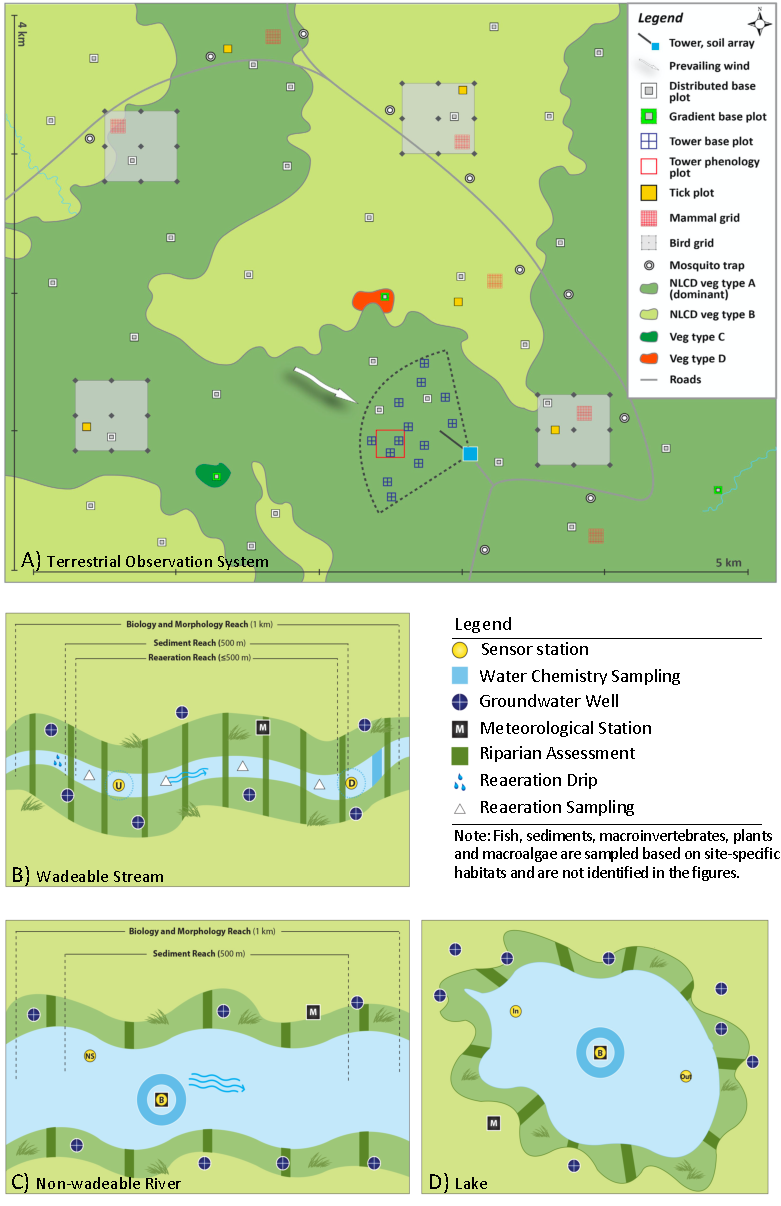
\includegraphics[width=0.95\linewidth]{/Users/dli/Github/neonDivData/manuscript/figures/fig_1} 

}

\caption{Generalized sampling schematics for Terrestrial Observation System (A) and Aquatic Observation System (B-D) plots. For Terrestrial Observation System (TOS) plots, Distributed, Tower, and Gradient plots, and locations of various sampling regimes, are presented via symbols. For Aquatic Observation System (AOS) plots, Wadeable streams, Non-wadeable streams, and Lake plots are shown in detail, with locations of sensors and different sampling regimes presented using symbols. Panel A was originally published in Thorpe et al. (2016).}\label{fig:Fig1Design}
\end{figure}



\begin{table}

\caption{\label{tab:dataMapping}Mapping NEON data products to ecocomDP formatted data packages with abundances \emph{standardized} to observation effort. IDs in the \texttt{L0\ to\ L1\ ecocomDP\ workflow\ ID} columns were used in the R package \texttt{ecocomDP} to standardize organismal data. Notes: *Bird counts are reported per taxon per ``cluster'' observed in each point count in the NEON data product and have not been further standardized to sampling effort because standard methods for modeling bird abundances are beyond the scope of this paper; ** plants percent cover value \texttt{NA} represents presence/absence data only; incidence rate per number of tests conducted is reported for tick pathogens.}
\centering
\resizebox{\linewidth}{!}{
\begin{tabular}[t]{>{\raggedright\arraybackslash}p{7.5em}>{\raggedright\arraybackslash}p{6em}>{\raggedright\arraybackslash}p{12em}>{\raggedright\arraybackslash}p{12em}>{\raggedright\arraybackslash}p{9em}>{\raggedright\arraybackslash}p{9em}}
\toprule
Taxon group & L0 dataset (NEON data product ID) & Version of NEON data used in this study & L0 to L1 ecocomDP workflow ID & Primary variable reported in ecocomDP observation table & Units\\
\midrule
\cellcolor{gray!6}{Algae} & \cellcolor{gray!6}{DP1.20166.001} & \href{https://doi.org/10.48443/3cvp-hw55}{\cellcolor{gray!6}{https://doi.org/10.48443/3cvp-hw55 and provisional data}} & \cellcolor{gray!6}{neon.ecocomdp.20166.001.001} & \cellcolor{gray!6}{cell density OR cells OR valves} & \cellcolor{gray!6}{cells/cm2 OR cells/mL}\\
Beetles & DP1.10022.001 & \href{https://doi.org/10.48443/tx5f-dy17}{https://doi.org/10.48443/tx5f-dy17 and provisional data} & neon.ecocomdp.10022.001.001 & abundance & count per trap day\\
\cellcolor{gray!6}{Birds*} & \cellcolor{gray!6}{DP1.10003.001} & \href{https://doi.org/10.48443/s730-dy13}{\cellcolor{gray!6}{https://doi.org/10.48443/s730-dy13 and provisional data}} & \cellcolor{gray!6}{neon.ecocomdp.10003.001.001} & \cellcolor{gray!6}{cluster size} & \cellcolor{gray!6}{count of individuals}\\
Fish & DP1.20107.001 & \href{https://doi.org/10.48443/17cz-g567}{https://doi.org/10.48443/17cz-g567 and provisional data} & neon.ecocomdp.20107.001.001 & abundance & catch per unit effort\\
\cellcolor{gray!6}{Herptiles} & \cellcolor{gray!6}{DP1.10022.001} & \href{https://doi.org/10.48443/tx5f-dy17}{\cellcolor{gray!6}{https://doi.org/10.48443/tx5f-dy17 and provisional data}} & \cellcolor{gray!6}{neon.ecocomdp.10022.001.002} & \cellcolor{gray!6}{abundance} & \cellcolor{gray!6}{count per trap day}\\
Macroinvertebrates & DP1.20120.001 & \href{https://doi.org/10.48443/855x-0n27}{https://doi.org/10.48443/855x-0n27 and provisional data} & neon.ecocomdp.20120.001.001 & density & count per square meter\\
\cellcolor{gray!6}{Mosquitoes} & \cellcolor{gray!6}{DP1.10043.001} & \href{https://doi.org/10.48443/9smm-v091}{\cellcolor{gray!6}{https://doi.org/10.48443/9smm-v091 and provisional data}} & \cellcolor{gray!6}{neon.ecocomdp.10043.001.001} & \cellcolor{gray!6}{abundance} & \cellcolor{gray!6}{count per trap hour}\\
Plants** & DP1.10058.001 & \href{https://doi.org/10.48443/abge-r811}{https://doi.org/10.48443/abge-r811 and provisional data} & neon.ecocomdp.10058.001.001 & percent cover & percent of plot area covered by taxon\\
\cellcolor{gray!6}{Small mammals} & \cellcolor{gray!6}{DP1.10072.001} & \href{https://doi.org/10.48443/j1g9-2j27}{\cellcolor{gray!6}{https://doi.org/10.48443/j1g9-2j27 and provisional data}} & \cellcolor{gray!6}{neon.ecocomdp.10072.001.001} & \cellcolor{gray!6}{count} & \cellcolor{gray!6}{unique individuals per 100 trap nights per plot per month}\\
Tick pathogens*** & DP1.10092.001 & \href{https://doi.org/10.48443/5fab-xv19}{https://doi.org/10.48443/5fab-xv19 and provisional data} & neon.ecocomdp.10092.001.001 & positivity rate & positive tests per pathogen per sampling event\\
\cellcolor{gray!6}{Ticks} & \cellcolor{gray!6}{DP1.10093.001} & \href{https://doi.org/10.48443/dx40-wr20}{\cellcolor{gray!6}{https://doi.org/10.48443/dx40-wr20 and provisional data}} & \cellcolor{gray!6}{neon.ecocomdp.10093.001.001} & \cellcolor{gray!6}{abundance} & \cellcolor{gray!6}{count per square meter}\\
Zooplankton & DP1.20219.001 & \href{https://doi.org/10.48443/qzr1-jr79}{https://doi.org/10.48443/qzr1-jr79 and provisional data} & neon.ecocomdp.20219.001.001 & density & count per liter\\
\bottomrule
\end{tabular}}
\end{table}

\hypertarget{terrestrial-organisms}{%
\subsection{Terrestrial Organisms}\label{terrestrial-organisms}}

\hypertarget{breeding-land-birds}{%
\subsubsection{Breeding Land Birds}\label{breeding-land-birds}}

\textbf{NEON Sampling Design} NEON designates breeding landbirds as ``smaller birds (usually exclusive of raptors and upland game birds) not usually associated with aquatic habitats'' (Ralph 1993, Thibault 2018). Most species observed are diurnal and include both resident and migrant species. Landbirds are surveyed via point counts in each of the 47 terrestrial sites (Thibault 2018). At most NEON sites, breeding landbird points are located in five to ten 3 \(\times\) 3 grids (Fig. \ref{fig:Fig1Design}), which are themselves located in representative (dominant) vegetation. Whenever possible, grid centers are co-located with distributed base plot centers. When sites are too small to support a minimum of five grids, separated by at least 250 m from edge to edge, point counts are completed at single points instead of grids. In these cases, points are located at the southwest corners of distributed base plots within the site. Five to 25 points may be surveyed depending on the size and spatial layout of the site, with exact point locations dictated by a stratified-random spatial design that maintains a 250 m minimum separation between points.

Surveys occur during one or two sampling bouts per season, at large and small sites respectively. Observers go to the specified points early in the morning and track birds observed during each minute of a 6-minute period, following a 2-minute acclimation period, at each point (Thibault 2018). Each point count contains species, sex, and distance to each bird (measured with a laser rangefinder except in the case of flyovers) seen or heard. Information relevant for subsequent modeling of detectability is also collected during the point counts (e.g., weather, detection method). The point count surveys for NEON were modified from the Integrated Monitoring in Bird Conservation Regions (IMBCR) field protocol for spatially-balanced sampling of landbird populations (Pavlacky Jr et al. 2017).

To protect species of concern, breeding landbird taxonomic IDs are `fuzzed,' whereby the data are provided by NEON with a taxonomic identification at one higher taxonomic level than where the protection occurs (Elmendorf and Brownlee 2018). For example, if a threatened Black-capped vireo (\emph{Vireo atricapilla}) is recorded by a NEON technician, the taxonomic identification is fuzzed to Vireo in the data. Rare, threatened and endangered species are those listed as such by federal and/or state agencies.

\textbf{Data Wrangling Decisions} The bird point count NEON data product (`DP1.10003.001') consists of a list of two associated data frames: \texttt{brd\_countdata} and \texttt{brd\_perpoint}. The former data frame contains information such as locations, species identities, and their counts. The latter data frame contains additional location information such as latitude and longitude coordinates and environmental conditions during the time of the observations. The separate data frames are linked by `eventID,' which refers to the location, date and time of the observation. To prepare the bird point count data for the L1 ecocomDP model, we first merged both data frames into one and then removed columns that are likely not needed for most community-level biodiversity analyses (e.g., observer names, etc.). The field \texttt{taxon\_id} in the R object \texttt{data\_bird} with the \texttt{neonDivData} data package consists of the standard AOU 4-letter species code, although \texttt{taxon\_rank} refers to eight potential levels of identification (class, family, genus, species, speciesGroup, subfamily, and subspecies). Users can decide which level is appropriate, for example one might choose to exclude all unidentified birds (taxon\_id = UNBI), where no further details are available below the class level (Aves sp.). The NEON sampling protocol has evolved over time, so users are advised to check whether the `samplingProtocolVersion' associated with bird point count data (`DP1.10003.001') fits their data requirements and subset as necessary. Older versions of protocols can be found at the \href{https://data.neonscience.org/documents/-/document_library_display/JEygRkSpUBoq/view/1883155?_110_INSTANCE_JEygRkSpUBoq_topLink=home\&_110_INSTANCE_JEygRkSpUBoq_delta1=20\&_110_INSTANCE_JEygRkSpUBoq_keywords=\&_110_INSTANCE_JEygRkSpUBoq_advancedSearch=false\&_110_INSTANCE_JEygRkSpUBoq_andOperator=true\&p_r_p_564233524_resetCur=false\&_110_INSTANCE_JEygRkSpUBoq_delta2=20\&_110_INSTANCE_JEygRkSpUBoq_cur2=1}{NEON document library}.

\hypertarget{ground-beetles-and-herp-bycatch}{%
\subsubsection{Ground Beetles and Herp Bycatch}\label{ground-beetles-and-herp-bycatch}}

\textbf{NEON Sampling Design} Ground beetle sampling is conducted via pitfall trapping, across 10 distributed plots at each NEON site. The original sampling design included the placement of a pitfall trap at each of the cardinal directions along the distributed plot boundary, for a total of four traps per plot and 40 traps per site. In 2018, sampling was reduced via the elimination of the North pitfall trap in each plot, resulting in 30 traps per site (LeVan et al. 2019b).

Beetle pitfall trapping begins when the temperature has been \textgreater4°C for 10 days in the spring and ends when temperatures dip below this threshold in the fall. Sampling occurs biweekly throughout the sampling season with no single trap being sampled more frequently than every 12 days (LeVan 2020a). After collection, the samples are separated into carabid species and bycatch.

Invertebrate bycatch is pooled to the plot level and archived. Vertebrate bycatch is sorted and identified by NEON technicians, then archived at the trap level. Carabid samples are sorted and identified by NEON technicians, after which a subset of carabid individuals are sent to be pinned and re-identified by an expert taxonomist. More details can be found in Hoekman et al. (2017) and LeVan et al. (2019b).

Pitfall traps and sampling methods are designed by NEON to reduce vertebrate bycatch (LeVan et al. 2019b). The pitfall cup is medium in size with a low clearance cover installed over the trap entrance to minimize large vertebrate bycatch. When a live vertebrate with the ability to move on its own volition is found in a trap, the animal is released. Live but morbund vertebrates are euthanized and collected along with deceased vertebrates. When ≥15 individuals of a vertebrate species are collected, cumulatively, within a single plot, NEON may initiate localized mitigation measures such as temporarily deactivating traps and removing all traps from the site for the remainder of the season. Thus, while herpetofaunal (herp) bycatch is present in many pitfall samples it is unclear how well these pitfall traps capture herp community structure and diversity - due to these active efforts to reduce vertebrate bycatch. Users of NEON herp bycatch data should be aware of these limitations.

\textbf{Data Wrangling Decisions} The beetle and herp bycatch data product identifier is `DDP1.10022.001.' Carabid samples are recorded and identified in a multi-step workflow wherein a subset of samples are passed on in each successive step. Individuals are first identified by the sorting technician after which a subset is sent on to be pinned. Some especially difficult individuals are not identified by technicians during sorting, instead being labelled ``other carabid.'' The identifications for those individuals are recorded with the pinning data. Any individuals for which identification is still uncertain are then verified by an expert taxonomist. There are a few cases where an especially difficult identification was sent to multiple expert taxonomists and they did not agree on a final taxon, these individuals were excluded from the data set at the recommendation of NEON staff.

Preference is given to expert identification whenever available. However, these differences in taxonomic expertise do not seem to cause systematic biases in estimating species richness across sites, but non-expert taxonomists are more likely to misidentify non-native carabid species (Egli et al. 2020). Beetle abundances are recorded for the sorted samples by NEON technicians. To account for individual samples that were later reidentified, the final abundance for a species is the original sorting sample abundance minus the number of individuals that were given a new ID.

Prior to 2018, \texttt{trappingDays} values were not included for many sites. Missing entries were calculated as the range from \texttt{setDate} through \texttt{collectDate} for each trap. We also accounted for a few plots for which \texttt{setDate} was not updated based on a previous collection event in the \texttt{trappingDays} calculations. To facilitate easy manipulation of data within and across bouts, a new \texttt{boutID} field was created to identify all trap collection events at a site in a bout. The original \texttt{EventID} field is intended to identify a bout, but has a number of issues that necessitates creation of a new ID. First, \texttt{EventID} does not correspond to a single collection date but rather all collections in a week. This is appropriate for the small number of instances when collections for a bout happen over multiple consecutive days (\textasciitilde5\% of bouts), but prevents analysis of bout patterns at the temporal scale of a weekday. The data here were updated so all entries for a bout correspond to the date (i.e., \texttt{collectDate}) on which the majority of traps are collected to maintain the weekday-level resolution with as high of fidelity as possible, while allowing for easy aggregation within bouts and \texttt{collectDate}'s. Second, there were a few instances in which plots within a site were set and collected on the same day, but have different \texttt{EventID}'s. These instances were all considered a single bout by our new \texttt{boutID}, which is a unique combination of \texttt{setDate}, \texttt{collectDate}, and \texttt{siteID}.

Herpetofaunal bycatch (amphibian and reptile) in pitfall traps were identified to species or the lowest taxonomic level possible within 24 h of recovery from the field. To process the herp bycatch NEON data we cleaned \texttt{trappingDays} and the other variables and added \texttt{boutID} as described above for beetles. The variable \texttt{sampleType} in the \texttt{bet\_sorting} table provides the type of animal caught in a pitfall trap as one of five types: `carabid,' `vert bycatch herp,' `other carabid,' `invert bycatch' and `vert bycatch mam.' We filtered the beetle data described above to only include the `carabid' and `other carabid' types. For herps, we only kept the \texttt{sampleType} of `vert bycatch herp.' Abundance data of beetles and herps bycatch were standardized to be the number of individuals captured per trap day.

\hypertarget{mosquitos}{%
\subsubsection{Mosquitos}\label{mosquitos}}

\textbf{NEON Sampling Design} Mosquito specimens are collected at 47 terrestrial sites across all NEON domains and the data are reported in NEON data product DP1.10043.001. Traps are distributed throughout each site according to a stratified-random spatial design used for all Terrestrial Observation System sampling, maintaining stratification across dominant (\textgreater5\% of total cover) vegetation types (LeVan 2020b). The number of mosquito traps placed in each vegetation type is proportional to its percent cover, until 10 total mosquito traps have been placed in the site. Mosquito traps are typically located within 30 m of a road to facilitate expedient sampling, and are placed at least 300 m apart to maintain independence.

Mosquito monitoring is divided into off-season and field season sampling (LeVan et al. 2019a). Off-season sampling begins after three consecutive zero-catch field sampling bouts have occurred, and represents a reduced sampling regime that is designed for the rapid detection of when the next field season should begin and to provide mosquito phenology data. Off-season sampling is conducted at three dedicated mosquito traps spread throughout each core site, while temperatures are \textgreater10 °C. Once per week, technicians deploy traps at dusk and then collect them at dawn the following day.

Field season sampling begins when the first mosquito is detected during off season sampling (LeVan et al. 2019a). Technicians deploy traps at all 10 dedicated mosquito trap locations per site. Traps remain out for a 24-hour period, or sampling bout, and bouts occur every two or four weeks at core and relocatable terrestrial sites, respectively. During the sampling bout, traps are serviced twice and yield one night-active sample, collected at dawn or about eight hours after the trap was set, and one day-active sample, collected at dusk or \textasciitilde16 hours after the trap was set. Thus, a 24-hour sampling bout yields 20 samples from 10 traps.

NEON collects mosquito specimens using Center for Disease Control (CDC) CO\textsubscript{2} light traps (LeVan et al. 2019a). These traps have been used by other public health and mosquito-control agencies for a half-century, so that NEON mosquito data align across NEON field sites and with existing long-term data sets. A CDC CO\textsubscript{2} light trap consists of a cylindrical insulated cooler that contains dry ice, a plastic rain cover attached to a battery powered light/fan assembly, and a mesh collection cup. During deployment, the dry ice sublimates and releases CO\textsubscript{2}. Mosquitoes attracted to the CO\textsubscript{2} bait are sucked into the mesh collection cup by the battery-powered fan, where they remain alive until trap collection.

Following field collection, NEON's field ecologists process, package, and ship the samples to an external lab where mosquitoes are identified to species and sex (when possible). A subset of identified mosquitoes are tested for infection by pathogens to quantify the presence/absence and prevalence of various arboviruses. Some mosquitoes are set aside for DNA barcode analysis as well as long-term archiving. Particularly rare or difficult to identify mosquito specimens are prioritized for DNA barcoding. More details can be found in LeVan et al. (2019a).

\textbf{Data Wrangling Decisions} The mosquito data product (\texttt{DP1.10043.001}) consists of four data frames: trapping data (\texttt{mos\_trapping}), sorting data (\texttt{mos\_sorting}), archiving data (\texttt{mos\_archivepooling}), and expert taxonomist processed data (\texttt{mos\_expertTaxonomistIDProcessed}). We first removed rows (records) with missing information about location, collection date, and sample or subsample ID for all data frames. We then merged all four data frames into one, wherein we only kept records for target taxa (i.e., targetTaxaPresent = ``Y'') with no known compromised sampling condition (i.e., sampleCondition = ``No known compromise''). We further removed a small number of records with species identified only to the family level; all remaining records were identified at least to the genus level. We estimated the total individual count per trap-hour for each species within a trap as \texttt{(individualCount/subsampleWeight)\ *\ totalWeight\ /\ trapHours}. We then removed columns that were not likely to be used for calculating biodiversity values.

\hypertarget{small-mammals}{%
\subsubsection{Small Mammals}\label{small-mammals}}

\textbf{NEON Sampling Design} NEON defines small mammals based on taxonomic, behavioral, dietary, and size constraints, and includes any rodent that is (1) nonvolant; (2) nocturnally active; (3) forages predominantly aboveground; and (4) has a mass \textgreater5 grams, but \textless\textasciitilde{} 500-600 grams (Thibault et al. 2019). In North America, this includes cricetids, heteromyids, small sciurids, and introduced murids, but excludes shrews, large squirrels, rabbits, or weasels, although individuals of these species may be incidentally captured.

Small mammals are collected at NEON sites using Sherman traps, identified to species in the field, marked with a unique tag, and released (Thibault et al. 2019). Multiple 90 m \(\times\) 90 m trapping grids are set up in each terrestrial field site within the dominant vegetation type. Each 90 m \(\times\) 90 m trapping grid contains 100 traps placed in a pattern with 10 rows and 10 columns set 10 m apart. Three of these 90 m \(\times\) 90 m grids per site are designated pathogen (as opposed to diversity) grids and additional blood sampling is conducted here.

Small mammal sampling occurs in bouts, with a bout comprised of three consecutive (or nearly consecutive) nights of trapping at each pathogen grid and one night of trapping at each diversity grid. The timing of sampling occurs within 10 days before or after the new moon. The number of bouts per year is determined by site type: core sites are typically trapped for six bouts per year (except for areas with shorter seasons due to cold weather), while relocatable sites are trapped for four bouts per year. More information can be found in Thibault et al. (2019).

\textbf{Data Wrangling Decisions} In the small mammal NEON data product (\texttt{DP1.10072.001}), records are stratified by NEON site, year, month, and day and represent data from both the diversity and pathogen sampling grids. Capture records were removed if they were not identified to genus or species (e.g., if the species name was denoted as `either/or' or as family name), or if their trap status is not ``5 - capture'' or ``4 - more than 1 capture in one trap.'' Abundance data for each plot and month combination were standardized to be the number of individuals captured per 100 trap nights.

\hypertarget{soil-microbes}{%
\subsubsection{Soil Microbes}\label{soil-microbes}}

\textbf{NEON Sampling Design} Soil samples are collected at ten 40 m \(\times\) 40 m NEON plots per site (Stanish et al. 2020). Four plots are within the tower airshed (tower plots), and six plots are distributed across the landscape (distributed plots). Within each plot, soils are sampled from three predetermined, randomly assigned XY coordinate locations, relative to the southwest corner of the plot. Soils are sampled by horizon, with organic (O) and mineral (M) material collected separately. During standard `microbes' bouts (most common), soils are taken from only the surface horizon (O if present, else M) - with a maximum depth of 30 ± 1 cm where possible. Every five years, during coordinated microbes/biogeochemistry bouts, soils are collected from both O and M horizons if both are present, and samples are processed separately for all downstream analyses.

Most NEON sites, except for the boreal/arctic sites, are sampled three times a year, once at peak vegetation greenness (``peak greenness bout'') and two other times bracketing the period capturing seasonal transitions (Stanish et al. 2020). This results in \textasciitilde10 plots \(\times\) 3 locations \(\times\) 1 or 2 horizons \(\times\) 3 bouts = 90 to 180 soil samples per site per year for most sites.

Sample timing and locations for soil microbes have changed in important ways since data collection began at NEON. From 2013 to the end of 2014, microbial analyses were performed on all soil samples at all sites. From January 2014 to September 2014, soil samples were pooled at the plot and horizon levels for some plots, to assess the ability of pooled data to provide information. Thus, a subset of analyses during this period reflect soils pooled to the per‐plot and per‐horizon level. This method was subsequently adopted, and from 2015 on soil samples from the same plot and for the same horizon type were pooled prior to analyses. 2015 saw an additional sampling design change, wherein microbial analyses were reduced to occur only once per year, during the period of peak greenness/productivity, at all sites. This change held until 2019, at which point microbial analyses were altered one last time to occur once per year, during the period of peak greenness/productivity, at one site per domain and during all coordinated bouts (every five years) at all sites.

\textbf{Data Wrangling Decisions} Unlike other NEON biodiversity data products, the soil microbial NEON data product (\texttt{DP1.10107.001}) requires significant pre-processing to go from raw sequence data to a community matrix, and the exact bioinformatics methods will vary depending on use case. Briefly, major decisions during this process will depend on whether users are working with fungal (ITS) or bacterial (16S) data, if the goal is to maximize read quality and taxonomic resolution vs.~number of reads retained through the quality filter process, and whether to remove or retain reverse complement reads for a merged sequence. The full description of a suggested bioinformatics pipeline, how to run sensitivity analyses on user-defined parameters, accompanying code, and vignettes are described in Qin et al.~in prep. At the end of the suggested bioinformatics pipeline, users will have a phyloseq object, which is a commonly-used format for sequence-based analysis software. The phyloseq object will contain a table of ASV (amplicon sequence variant) sequences, a table of taxonomic assignments, and soil chemical and physical data associated with corresponding sample locations and sampling bouts.

Note that NEON provides both ITS and 16S marker gene sequence data for soil, benthic, and surface water microbes in data products DP1.10108.001, DP1.20280.001, and DP1.20282.001, respectively. Based on the input from the potential data user community, NEON staff scientists have recently developed an in-house bioinformatics pipeline to produce associated derived soil, benthic, and surface water microbe community composition data products, which are published as DP1.10081.001, DP1.20086.001, and DP1.20141.001, respectively. However, at the time of writing this, the completed community composition data products have not been fully published; thus, they focus on the soil microbial marker gene sequences data product (DP1.10108.001), which has the most extensive spatial and temporal coverage for data availability out of the marker gene sequence data products.

\hypertarget{terrestrial-plants}{%
\subsubsection{Terrestrial Plants}\label{terrestrial-plants}}

\textbf{NEON Sampling Design} NEON plant diversity sampling is completed once or twice per year (one or two `bouts') in multiscale, 400 m\textsuperscript{2} (20 m \(\times\) 20 m) plots (Barnett 2019). Each multiscale plot is subdivided into four 100 m\textsuperscript{2} (10 m \(\times\) 10 m) subplots that each encompass one or two sets of 10 m\textsuperscript{2} (3.16 m \(\times\) 3.16 m) subplots within which a 1 m\textsuperscript{2} (1 m \(\times\) 1 m) subplot is nested. The percent cover of each plant species is estimated visually in the 1 m\textsuperscript{2} subplots, while only species presences are documented in the 10 m\textsuperscript{2} and 100 m\textsuperscript{2} subplots.

To estimate plant percent cover by species, technicians record this value for all species in a 1 m\textsuperscript{2} subplot (Barnett 2019). Next, the remaining 9 m\textsuperscript{2} area of the associated 10 m\textsuperscript{2} subplot is searched for the presence of species. The process is repeated if there is a second 1 and 10 m\textsuperscript{2} nested pair in the specific 100 m\textsuperscript{2} subplot. Next, the remaining 80 m\textsuperscript{2} area is searched for the presence of species; data can be aggregated for a complete list of species present at the 100 m\textsuperscript{2} subplot scale. Data for all four 100 m\textsuperscript{2} subplots represent indices of species at the 400 m\textsuperscript{2} plot scale. In most cases, species encountered in a nested, finer scale, subplot are not rerecorded in any corresponding larger subplot - in order to avoid duplication. Plant species are occasionally recorded more than once, however, when data are aggregated across all nested subplots within each 400 m\textsuperscript{2} plot, and these require removal from the dataset. More details about the sampling design can be found in Barnett et al. (2019).

NEON manages plant taxonomic entries with a master taxonomy list that is based on the community standard, where possible. Using this list, synonyms for a given species are converted to the currently used name. The master taxonomy for plants is the USDA PLANTS Database (USDA, NRCS. 2014. \url{https://plants.usda.gov}), and the portions of this database included in the NEON plant master taxonomy list are those pertaining to native and naturalized plants present within the NEON sampling area. A sublist for each NEON domain includes those species with ranges that overlap the domain as well as nativity designations - introduced or native - in that part of the range. If a species is reported at a location outside of its known range, and the record proves reliable, the master taxonomy list is updated to reflect the distribution change. For more details on plant taxonomic handling, see Barnett (2019). For more on the NEON plant master taxonomy list see NEON.DOC.014042 (\url{https://data.neonscience.org/api/v0/documents/NEON.DOC.014042vK}).

\textbf{Data Wrangling Decisions} In the plant presence and percent cover NEON data product (\texttt{DP1.10058.001}) sampling at the 1 m \(\times\) 1 m scale also includes observations of abiotic and non-target species ground cover (i.e., soil, water, downed wood), so we removed records with \texttt{divDataType} as ``otherVariables.'' We also removed records whose \texttt{targetTaxaPresent} is \texttt{N} (i.e., a non-target species). Additionally, for all spatial resolutions (i.e., 1 m\textsuperscript{2}, 10 m\textsuperscript{2}, and 100 m\textsuperscript{2} data), any record lacking information critical for combining data within a plot and for a given sampling bout (i.e., \texttt{plotID}, \texttt{subplotID}, \texttt{boutNumber}, \texttt{endDate}, or \texttt{taxonID}) was dropped from the dataset. Furthermore, records without a definitive genus or species level \texttt{taxonID} (i.e., those representing unidentified morphospecies) were not included. To combine data from different spatial resolutions into one data frame, we created a pivot column entitled \texttt{sample\_area\_m2} (with possible values of 1, 10, and 100). Because of the nested sampling design of the plant data, to capture all records within a subplot at the 100 m\textsuperscript{2} scale, we incorporated all data from both the 1 m\textsuperscript{2} and 10 m\textsuperscript{2} scales for that subplot. Similarly, to obtain all records within a plot at the 400 m\textsuperscript{2} scale, we included all data from that plot. Species abundance information was only recorded as area coverage within 1 m by 1 m subplots; however, users may use the frequency of a species across subplots within a plot or plots within a site as a proxy of its abundance if needed.

\hypertarget{ticks-and-tick-pathogens}{%
\subsubsection{Ticks and Tick Pathogens}\label{ticks-and-tick-pathogens}}

\textbf{NEON Sampling Design} Tick sampling occurs in six distributed plots at each site, which are randomly chosen in proportion to NLCD land cover class (LeVan et al. 2019c). Ticks are sampled by walking the perimeter of a 40 m \(\times\) 40 m plot using a 1 m \(\times\) 1 m drag cloth. Ideally, 160 meters are sampled (shortest straight line distance between corners), but the cloth can be dragged around obstacles if a straight line is not possible. Acceptable total sampling area is between 80 and 180 m per plot. The cloth can also be flagged over vegetation when the cloth cannot be dragged across it. Ticks are collected from the cloth and technicians' clothing at appropriate intervals, depending on vegetation density, and at every corner of the plot. Specimens are immediately transferred to a vial containing 95\% ethanol.

Onset and offset of tick sampling coincides with phenological milestones at each site, beginning within two weeks of the onset of green-up and ending within two weeks of vegetation senescence (LeVan et al. 2019c). Sampling bouts are only initiated if the high temperature on the two consecutive days prior to planned sampling was \textgreater0°C. Early season sampling is conducted on a low intensity schedule, with one sampling bout every six weeks. When more than five ticks of any life stage have been collected within the last calendar year at a site, sampling switches to a high intensity schedule at the site - with one bout every three weeks. A site remains on the high intensity schedule until fewer than five ticks are collected within a calendar year, then sampling reverts back to the low intensity schedule.

Ticks are sent to an external facility for identification to species, life stage, and sex (LeVan et al. 2019c). A subset of nymphal ticks are additionally sent to a pathogen testing facility. \emph{Ixodes} species are tested for \emph{Anaplasma phagocytophilum}, \emph{Babesia microti}, \emph{Borrelia burgdorferi} sensu lato, \emph{Borrelia miyamotoi}, \emph{Borrelia mayonii}, other \emph{Borrelia} species (\emph{Borrelia} sp.), and a \emph{Ehrlichia} muris-like agent (Pritt et al. 2017). \emph{Non-Ixodes} species are tested for \emph{Anaplasma phagocytophilum}, \emph{Borrelia lonestari} (and other undefined \emph{Borrelia} species), \emph{Ehrlichia chaffeensis}, \emph{Ehrlichia ewingii}, \emph{Francisella tularensis}, and \emph{Rickettsia rickettsii}. Additional information about tick pathogen testing can be found in the Tick Pathogen Testing SOP (\url{https://data.neonscience.org/api/v0/documents/UMASS_LMZ_tickPathogens_SOP_20160829}) for the NEON Tick-borne Pathogen Status data product.

\textbf{Data Wrangling Decisions} The tick NEON data product (\texttt{DP1.10093.001}) consists of two dataframes: `tck\_taxonomyProcessed' hereafter referred to as `taxonomy data' and `tck\_fielddata' hereafter referred to as `field data.' Users should be aware of some issues related to taxonomic ID. Counts assigned to higher taxonomic levels (e.g., at the order level \emph{Ixodida}; IXOSP2) are not the sum of lower levels; rather they represent the counts of individuals that could not reliably be assigned to a lower taxonomic unit. Samples that were not identified in the lab were assigned to the highest taxonomic level (order \emph{Ixodida}; IXOSP2). However, users could make an informed decision to assign these ticks to the most probable group if a subset of individuals from the same sample were assigned to a lower taxonomy.

To clean the tick data, we first removed surveys and samples not meeting quality standards. In the taxonomy data, we removed samples where sample condition was not listed as ``OK'' (\textless1\% of records). In the field data, we removed records where samples were not collected due to logistical concerns (10\%). We then combined male and female counts in the taxonomy table into one ``adult'' class. The taxonomy table was re-formatted so that every row contained a sampleID and counts for each species life-stages were separate columns (i.e., ``wide format''). Next, we joined the field data to the taxonomy data, using the sample ID to link the two tables. When joining, we retained field records where no ticks were found in the field and thus there were no associated taxonomy data. In drags where ticks were not found, counts were given zeros. All counts were standardized by area sampled.

Prior to 2019, both field surveyors and laboratory taxonomists enumerated each tick life-stage; consequently, in the joined dataset there were two sets of counts (``field counts'' and ``lab counts''). However, starting in 2019, counts were performed by taxonomists rather than field surveyors. Field surveys conducted after 2019 no longer have field counts. Users of tick abundance data should be aware that this change in protocol has several implications for data wrangling and for analysis. First, after 2019, tick counts are no longer published at the same time as field survey data. Subsequently, some field records from the most recent years have tick presence recorded (targetTaxaPresent = ``Y''), but do not yet have associated counts or taxonomic information and so the counts are still listed as \texttt{NA}. Users should be aware that counts of zero are therefore published earlier than positive counts. We strongly urge users to filter data to those years where there are no counts pending.

The second major issue is that in years where both field counts and lab counts were available, they did not always agree (8\% of records). In cases of disagreement, we generally used lab counts in the final abundance data, because this is the source of all tick count data after 2019 and because life-stage identification was more accurate. However, there were a few exceptions where we used field count data. In some cases, only a subsample of a certain life-stage was counted in the lab, which resulted in higher field counts than lab counts. In this case, we assigned the additional un-identified individuals (e.g., the difference between the field and lab counts) to the order level (IXOSP2). If quality notes from NEON described ticks being lost in transit, we also added the additional lost individuals to the order level. There were some cases (\textless1\%) where the field counts were greater than lab counts by more than 20\% and where the explanation was not obvious; we removed these records.We note that the majority of samples (\textasciitilde85\%) had no discrepancies between the lab or field, therefore this process could be ignored by users whose analyses are not sensitive to exact counts.

The tick pathogen NEON data product (\texttt{DP1.10092.001}) consists of two dataframes: \texttt{tck\_pathogen} hereafter referred to as `pathogen data' and \texttt{tck\_pathogenqa} hereafter referred to as `quality data.' First, we removed any samples that had flagged quality checks from the quality data and removed any samples that did not have a positive DNA quality check from the pathogen data. Although the original online protocol aimed to test 130 ticks per site per year from multiple tick species, the final sampling decision was to extensively sample IXOSCA, AMBAME, and AMBSP species only because IXOPAC and \emph{Dermacentor} nymph frequencies were too rare to generate meaningful pathogen data. \emph{Borrelia burgdorferi} and \emph{Borrelia burgdorferi sensu lato} tests were merged, since the former was an incomplete pathogen name and refers to \emph{B. burgdorferi sensu lato} as opposed to \emph{sensu stricto} (Rudenko et al. 2011). Tick pathogen data are presented as positivity rate calculated as number positive tests per number of tests conducted for a given pathogen on ticks collected during a given sampling event.

\hypertarget{aquatic-organisms}{%
\subsection{Aquatic Organisms}\label{aquatic-organisms}}

\hypertarget{aquatic-macroinvertebrates}{%
\subsubsection{Aquatic macroinvertebrates}\label{aquatic-macroinvertebrates}}

\textbf{NEON Sampling Design} Aquatic macroinvertebrate sampling occurs three times/year at wadeable stream, river, and lake sites from spring through fall. Timing of sampling is site-specific and based on historical hydrological, meteorological, and phenological data including dates of known ice cover, growing degree days, and green up and brown down (Cawley et al. 2016). Samplers vary by habitat and include Surber, Hess, hand corer, modified kicknet, D-frame sweep, and petite ponar samplers (Parker 2019). Stream sampling occurs throughout the 1 km permitted reach in wadeable areas of the two dominant habitat types. Lake sampling occurs with a petite ponar near buoy, inlet, and outlet sensors, and D-frame sweeps in wadeable littoral zones. Riverine sample collections in deep waters or near instrument buoys are made with a petite ponar, and in littoral areas are made with a D-frame sweep or large-woody debris sampler. In the field, samples are preserved in pure ethanol, and later in the domain support facility, glycerol is added to prevent the samples from becoming brittle. Samples are shipped from the domain facility to a taxonomy lab for sorting and identification to lowest possible taxon (e.g., genus or species) and counts of each taxon per size are made to the nearest mm.

\textbf{Data Wrangling Decisions} Aquatic macroinvertebrate data contained in the NEON data product \texttt{DP1.20120.001} are subsampled and identified to the lowest practical taxonomic level, typically genus, by expert taxonomists in the \texttt{inv\_taxonomyProcessed} table, measured to the nearest mm size class, and counted. Taxonomic naming has been standardized in the \texttt{inv\_taxonomyProcessed} file, according to NEON's master taxonomy (\url{https://data.neonscience.org/taxonomic-lists}), removing any synonyms. We calculated macroinvertebrate density by dividing \texttt{estimatedTotalCount} (which includes the corrections for subsampling in the taxonomy lab) by \texttt{benthicArea} from the \texttt{inv\_fieldData} table to return count per square meter of stream, lake, or river bottom (Chesney et al. 2021).

\hypertarget{microalgae-periphyton-and-phytoplankton}{%
\subsubsection{MicroAlgae (Periphyton and Phytoplankton)}\label{microalgae-periphyton-and-phytoplankton}}

\textbf{NEON Sampling Design} NEON collects periphyton samples from natural surface substrata (i.e., cobble, silt, woody debris) over a 1 km reach in streams and rivers, and in the littoral zone of lakes. Various collection methods and sampler types are used, depending on substrate (Parker 2020). In lakes and rivers, periphyton are also collected from the most dominant substratum type in three areas within the littoral (i.e., shoreline) zone. Prior to 2019, littoral zone periphyton sampling occurred in five areas.

NEON collects three phytoplankton samples per sampling date using Kemmerer or Van Dorn samplers. In rivers, samples are collected near the sensor buoy and at two other deep-water points in the main channel. For lakes, phytoplankton are collected near the central sensor buoy as well as at two littoral sensors. Where lakes and rivers are stratified, each phytoplankton sample is a composite from one surface sample, one sample from the metalimnion (i.e., middle layer), and one sample from the bottom of the euphotic zone. For non-stratified lakes and non-wadeable streams, each phytoplankton sample is a composite from one surface sample, one sample just above the bottom of the euphotic zone, and one mid-euphotic zone sample - if the euphotic zone is \textgreater{} 5 m deep.

All microalgae sampling occurs three times per year (i.e., spring, summer, and fall bouts) in the same sampling bouts as aquatic macroinvertebrates and zooplankton. In wadeable streams, which have variable habitats (e.g., riffles, runs, pools, step pools), three periphyton samples are collected per bout in the dominant habitat type (five samples collected prior to 2019) and three per bout in the second most dominant habitat type. No two samples are collected from the sample habitat unit (i.e., the same riffle).

Samples are processed at the domain support facility and separated into subsamples for taxonomic analysis or for biomass measurements. Aliquots shipped to an external facility for taxonomic determination are preserved in glutaraldehyde or Lugol's iodine (before 2021). Aliquots for biomass measurements are filtered onto glass-fiber filters and processed for ash-free dry mass.

\textbf{Data Wrangling Decisions} The periphyton, seston, and phytoplankton NEON data product (\texttt{DP1.20166.001}) contains three dataframes for algae containing information on algae taxonomic identification, biomass and related field data, which are hereafter referred to as \texttt{alg\_tax\_long}, \texttt{alg\_biomass} and \texttt{alg\_field\_data}. Algae within samples are identified to the lowest possible taxonomic resolution, usually species, by contracting laboratory taxonomists. Some specimens can only be identified to the genus or even class level, depending on the condition of the specimen. Ten percent of all samples are checked by a second taxonomist and are noted in the \texttt{qcTaxonomyStatus}. Taxonomic naming has been standardized in the \texttt{alg\_tax\_long} files, according to NEON's master taxonomy, removing nomenclatural synonyms. Abundance and cell/colony counts are determined for each taxon of each sample with counts of cells or colonies that are either corrected for sample volume or not (as indicated by algalParameterUnit = `cellsperBottle').

We corrected sample units of \texttt{cellsperBottle} to density (Parker and Vance 2020). First, we summed the preservative volume and the lab's recorded sample volume for each sample (from the \texttt{alg\_biomass} file) and combined that with the \texttt{alg\_tax\_long} file using \texttt{sampleID} as a common identifier. Where samples in the \texttt{alg\_tax\_long} file were missing data in the \texttt{perBottleSampleVolume} field (measured after receiving samples at the external laboratory), we estimated the sample volume using NEON domain lab sample volumes (measured prior to shipping samples to the external laboratory). With this updated file, we combined it with \texttt{alg\_field\_data} to have the related field conditions, including benthic area sampled for each sample. \texttt{parentSampleID} was used for \texttt{alg\_field\_data} to join to the \texttt{alg\_biomass} file's \texttt{sampleID} as \texttt{alg\_field\_data} only has \texttt{parentSampleID}. We then calculated cells per milliliter for the uncorrected taxon of each sample, dividing \texttt{algalParameterValue} by the updated sample volume. Benthic sample results are expressed in terms of area (i.e., multiplied by the field sample volume, divided by benthic area sampled), in square meters. The final abundance units are either cells/mL (phytoplankton and seston samples) or cells/m\textsuperscript{2} for benthic samples.

The \texttt{sampleIDs} are child records of each \texttt{parentSampleID} that will be collected as long as sampling is not impeded (i.e., ice covered or dry). In the \texttt{alg\_biomass} file, there should be only a single entry for each \texttt{parentSampleID}, \texttt{sampleID}, and \texttt{analysisType}. Most often, there were two \texttt{sampleID}'s per \texttt{parentSampleID} with one for ash-free dry mass (AFDM) and taxonomy (analysis types). For the creation of the observation table with standardized counts, we used only records from the \texttt{alg\_biomass} file with the \texttt{analysisType} of taxonomy. In \texttt{alg\_tax\_long}, there are multiple entries for each \texttt{sampleID} for each taxon by \texttt{scientificName} and \texttt{algalParameter}.

\hypertarget{fish}{%
\subsubsection{Fish}\label{fish}}

\textbf{NEON Sampling Design} Fish sampling is carried out across 19 of the NEON eco-climatic domains, occuring in a total of 23 lotic (stream) and five lentic (lake) sites. In lotic sites, up to 10 non-overlapping reaches, each 70 to 130 m long, are designated within a 1 km section of stream (Jensen et al. 2019a). These include three constantly sampled `fixed' reaches, which encompass all representative habitats found within the 1 km stretch, and seven `random' reaches that are sampled on a rotating schedule. In lentic sites, 10 pie-shaped segments are established, with each segment ranging from the riparian zone into the lake center, therefore effectively capturing both nearshore and offshore habitats (Jensen et al. 2019b). Three of the 10 segments are fixed and are surveyed twice a year, and the remaining segments are random and are sampled rotationally. The spatial layouts of these sites are designed to capture spatial and temporal heterogeneity in the aquatic habitats.

Lotic sampling occurs at three fixed and three random reaches per sampling bout, and there are two bouts per year - one in spring and one in fall. During each bout, the fixed reaches are sampled via a three-pass electrofishing depletion approach (Moulton II et al. 2002, Peck et al. 2006) while the random reaches being sampled are done so with a single-pass depletion approach. Which random reaches are surveyed depends on the year, with three of the random reaches sampled every other year. All sampling occurs during daylight hours, with each sampling bout completed within five days and with a minimum two-week gap in between two successive sampling bouts. The initial sampling date is determined using site-specific historical data on ice melting, water temperature (or accumulated degree days), and riparian peak greenness.

The lentic sampling design is similar to that discussed above, with fixed segments being sampled twice per year and random segments sampled twice per year on a rotational basis (i.e., each random segment is not sampled every year). Lentic sampling is conducted using three gear types, with backpack electrofishing and mini-fyke nets near the shoreline and gill nets in deeper waters. Backpack electrofishing is done on a 4 m \(\times\) 25 m reach near the shoreline via a three-pass (for fixed segments) or single-pass (for random segments) electrofishing depletion approach (Moulton II et al. 2002, Peck et al. 2006). All three passes in a fixed sampling segment are completed on the same night, with ≤30 minutes between successive passes. Electrofishing begins within 30 minutes of sunset and ceases within 30 minutes of sunrise, with a maximum of five passes per sampling bout. A single gill net is also deployed within all segments being sampled, both fixed and random, for 1-2 hours in either the morning or early afternoon. Finally, a fyke (Baker et al. 1997) or mini-fyke net is deployed at each fixed or random segments, respectively. Fyke nets are positioned before sunset and recovered after sunrise on the following day. Precise start and end times for electrofishing and net deployments are documented by NEON technicians at the time of sampling.

In all surveys, captured fish are identified to the lowest practical taxonomic level, and morphometrics (i.e., body mass and body length) are recorded for 50 individuals of each taxon before releasing. Relative abundance for each fish taxon is also recorded by direct enumeration (up to first 50 individuals) or estimation by bulk counts (\textgreater50 individuals, i.e., by placing fish of a given taxon into a dip net (i.e., net scoop), counting the total number of specimens in the dip net, and then multiplying the total number of scoops of captured fish by the counts from the first scoop).

\textbf{Data Wrangling Decisions} Fish sampled via both electrofishing and trapping are identified at variable taxonomic resolutions (as fine as subspecies level) in the field. Most identifications are made to the species or genus level by a single field technician for a given bout per site. Sampled fish are identified, measured, weighed, and then released back to the site of capture. If field technicians are unable to identify to the species level, such specimens are identified to the finest possible taxonomic resolution or assigned a morphospecies with a coarse-resolution identification. The standard sources consulted for identification and a qualifier for identification validity are also documented in the \texttt{fsh\_perFish} table. The column \texttt{bulkFishCount} of the \texttt{fsh\_bulkCount} table records relative abundance for each species or the alternative next possible taxon level (specified in the column \texttt{scientificName}).

Fish data (taxonomic identification and relative abundance) are recorded per each sampling reach in streams or per segment in lakes in each bout and documented in the \texttt{fsh\_perFsh} table (Monahan et al. 2020). The column \texttt{eventID} uniquely identifies the sampling date of the year, the specific site within the domain, a reach/segment identifier, the pass number (i.e., number of electrofishing passes or number of net deployment efforts), and the survey method. The \texttt{eventID} column helps tie all fish data with stream reach/lake segment data or environmental data (i.e., water quality data) and sampling effort data (e.g., electrofishing and net set time). A \texttt{reachID} column provided in the \texttt{fsh\_perPass} table uniquely identifies surveys done per stream reach or lake segment. The \texttt{reachID} is nested within the \texttt{eventID} as well. We used \texttt{eventID} as a nominal variable to uniquely identify different sampling events and to join different, stacked fish data files as described below.

The fish NEON data product (\texttt{DP1.20107.001}) consists of \texttt{fsh\_perPass}, \texttt{fsh\_fieldData}, \texttt{fsh\_bulkCount}, \texttt{fsh\_perFish,} and the complete taxon table for fish, for both stream and lake sites. To join all reach-scale data, we first joined the \texttt{fsh\_perPass} with \texttt{fsh\_fieldData}, and eliminated all bouts where sampling was untenable. Subsequently, we joined the reach-scale table with \texttt{fsh\_perFsh} to add individual fish counts and fish measurements. Then, to add bulk counts, we joined the reach-scale table with \texttt{fsh\_bulkCount} datasets, and subsequently added \texttt{taxonRank} which included the taxonomic resolution into the bulk-processed table. Afterward, both individual-level and bulk-processed datasets were appended into a single table. To include samples where no fish were captured, we filtered the \texttt{fsh\_perPass} table retaining records where target taxa (fish) were absent, joined it with \texttt{fsh\_fieldData}, and finally merged it with the table that contained both bulk-processed and individual-level data. For each finer-resolution taxon in the individual-level dataset, we considered the relative abundance as one since each row represented a single individual fish. Whenever possible, we substituted missing data by cross-referencing other data columns, omitted completely redundant data columns, and retained records with genus- and species-level taxonomic resolution. For the appended dataset, we also calculated the relative abundance for each species per sampling reach or segment at a given site. To calculate species-specific catch per unit effort (CPUE), we normalized the relative abundance by either average electrofishing time (i.e., \texttt{efTime}, \texttt{efTime2}) or trap deployment time (i.e., the difference between \texttt{netEndTime} and \texttt{netSetTime}). For trap data, we assumed that size of the traps used, water depths, number of netters used, and the reach lengths (a significant proportion of bouts had reach lengths missing) to be comparable across different sampling reaches and segments.

\hypertarget{zooplankton}{%
\subsubsection{Zooplankton}\label{zooplankton}}

\textbf{NEON Sampling Design} Zooplankton samples are collected at seven NEON lake sites across four domains. Zooplankton samples are collected at the buoy sensor set (deepest location in the lake) and at the two nearshore sensor sets using a vertical tow net for locations deeper than 4 m and a Schindler trap for locations shallower than 4 m (Parker and Roehm 2019). This results in three samples collected per sampling day. Samples are preserved with ethanol in the field and shipped from the domain facility to a taxonomy lab for sorting and identification to lowest possible taxon (e.g., genus or species) and counts of each taxon per size are made to the nearest mm.

\textbf{Data Wrangling Decisions} The NEON zooplankton data product (\texttt{DP1.20219.001}) consists of dataframes for taxonomic identification and related field data (Parker and Scott 2020). Zooplankton in NEON samples are identified at contracting labs to the lowest possible taxonomic resolution, usually genus, however some specimens can only be identified to the family (or even class) level, depending on the condition of the specimen. Ten percent of all samples are checked by two taxonomists and are noted in the \texttt{qcTaxonomyStatus} column. The taxonomic naming has been standardized in the \texttt{zoo\_taxonomyProcessed} table, according to NEON's master taxonomy, removing any synonyms. Density was calculated using \texttt{adjCountPerBottle} and \texttt{towsTrapsVolume} to correct count data to ``count per liter.''

\hypertarget{results-or-how-to-get-and-use-standardized-neon-organismal-data}{%
\section{Results (or how to get and use standardized NEON organismal data)}\label{results-or-how-to-get-and-use-standardized-neon-organismal-data}}

All cleaned and standardized datasets can be obtained from the R package \texttt{neonDivData} and from the EDI data repository (). Note that \texttt{neonDivData} included both stable and provisional data released by NEON while the data repository in EDI only included stable datasets. If users want to change some of the decisions to wrangle the data differently, they can find the code in the R package \texttt{ecocomDP} and modify them for their own purposes.

The data package \texttt{neonDivData} can be installed from Github. Installation instructions can be found on the Github webpage (\url{https://github.com/daijiang/neonDivData}). Table \ref{tab:dataSummary} shows the brief summary of all data objects. To get data for a specific taxonomic group, we can just call the objects in the \texttt{R\ object} column in Table \ref{tab:dataSummary}. Such data products include cleaned (and standardized if needed) occurrence data for the taxonomic groups covered and are equivalent to the ``observation'' table of the ecocomDP data format. If environmental information were provided by NEON for some taxonomic groups, they are also included in these data objects. Information such as latitude, longitude, and elevation for all taxonomic groups were saved in the \texttt{neon\_location} object of the R package, which is equivalent to the ``sampling\_location'' table of the ecocomDP data format. Information about species scientific names of all taxonomic groups were saved in the \texttt{neon\_taxa} object, which is equivalent to the ``taxon'' table of the ecocomDP data format.



\begin{table}

\caption{\label{tab:dataSummary}Summary of data products included in this study (as of 28 March, 2021). Users can call the R objects in the \texttt{R\ object} column from the R data package \texttt{neonDivData} to get the standardized data for specific taxonomic groups.}
\centering
\resizebox{\linewidth}{!}{
\begin{tabular}[t]{llrrll}
\toprule
Taxon group & R object & N species & N sites & Start date & End date\\
\midrule
\cellcolor{gray!6}{Algae} & \cellcolor{gray!6}{data\_algae} & \cellcolor{gray!6}{1946} & \cellcolor{gray!6}{33} & \cellcolor{gray!6}{2014-07-02} & \cellcolor{gray!6}{2019-07-15}\\
Beetles & data\_herp\_bycatch & 756 & 47 & 2013-07-03 & 2020-10-13\\
\cellcolor{gray!6}{Birds} & \cellcolor{gray!6}{data\_bird} & \cellcolor{gray!6}{541} & \cellcolor{gray!6}{47} & \cellcolor{gray!6}{2015-05-13} & \cellcolor{gray!6}{2020-07-20}\\
Fish & data\_fish & 147 & 28 & 2016-03-29 & 2020-12-03\\
\cellcolor{gray!6}{Herptiles} & \cellcolor{gray!6}{data\_herp\_bycatch} & \cellcolor{gray!6}{128} & \cellcolor{gray!6}{41} & \cellcolor{gray!6}{2014-04-02} & \cellcolor{gray!6}{2020-09-29}\\
Macroinvertebrates & data\_macroinvertebrate & 1330 & 34 & 2014-07-01 & 2020-08-12\\
\cellcolor{gray!6}{Mosquitoes} & \cellcolor{gray!6}{data\_mosquito} & \cellcolor{gray!6}{128} & \cellcolor{gray!6}{47} & \cellcolor{gray!6}{2014-04-09} & \cellcolor{gray!6}{2020-06-16}\\
Plants & data\_plant & 6197 & 47 & 2013-06-24 & 2020-10-23\\
\cellcolor{gray!6}{Small mammals} & \cellcolor{gray!6}{data\_small\_mammal} & \cellcolor{gray!6}{145} & \cellcolor{gray!6}{46} & \cellcolor{gray!6}{2013-06-19} & \cellcolor{gray!6}{2020-11-20}\\
Tick pathogens & data\_tick\_pathogen & 12 & 15 & 2014-04-17 & 2018-10-03\\
\cellcolor{gray!6}{Ticks} & \cellcolor{gray!6}{data\_tick} & \cellcolor{gray!6}{19} & \cellcolor{gray!6}{46} & \cellcolor{gray!6}{2014-04-02} & \cellcolor{gray!6}{2020-10-06}\\
Zooplankton & data\_zooplankton & 157 & 7 & 2014-07-02 & 2020-07-22\\
\bottomrule
\end{tabular}}
\end{table}

To demonstrate the use of data packages, we used \texttt{data\_plant} to quickly visualize the distribution of species richness of plants across all NEON sites (Fig. \ref{fig:Fig2Map}). To show how easy it is to get site level species richness, we presented the code used to generate the data for Fig. \ref{fig:Fig2Map} below.

\begin{Shaded}
\begin{Highlighting}[]
\FunctionTok{library}\NormalTok{(dplyr)}
\FunctionTok{library}\NormalTok{(neonDivData)}
\CommentTok{\# get species richness at each site}
\NormalTok{sp\_rich\_plant }\OtherTok{=}\NormalTok{ data\_plant }\SpecialCharTok{\%\textgreater{}\%}
  \FunctionTok{group\_by}\NormalTok{(siteID) }\SpecialCharTok{\%\textgreater{}\%}
  \FunctionTok{summarise}\NormalTok{(}\AttributeTok{nspp =} \FunctionTok{n\_distinct}\NormalTok{(taxon\_id), }\AttributeTok{.groups =} \StringTok{"drop"}\NormalTok{)}
\CommentTok{\# get latitude and longitude of all sites}
\NormalTok{sp\_rich\_plant }\OtherTok{=} \FunctionTok{left\_join}\NormalTok{(sp\_rich\_plant,}
                          \FunctionTok{filter}\NormalTok{(neon\_location, location\_id }\SpecialCharTok{\%in\%}\NormalTok{ data\_plant}\SpecialCharTok{$}\NormalTok{location\_id) }\SpecialCharTok{\%\textgreater{}\%}
                            \CommentTok{\# each site has multiple plots with slightly different lat/long}
                            \FunctionTok{group\_by}\NormalTok{(siteID) }\SpecialCharTok{\%\textgreater{}\%}
                            \FunctionTok{summarise}\NormalTok{(}\AttributeTok{latitude =} \FunctionTok{mean}\NormalTok{(latitude),}
                                      \AttributeTok{longitude =} \FunctionTok{mean}\NormalTok{(longitude),}
                                      \AttributeTok{.groups =} \StringTok{"drop"}\NormalTok{),}
                          \AttributeTok{by =} \StringTok{"siteID"}\NormalTok{)}
\end{Highlighting}
\end{Shaded}

Figure \ref{fig:Fig2Map} shows the utility of the data package for exploring macroecological patterns at the NEON site level. One of the most well known and studied macroecological patterns is the latitudinal biodiversity gradient, wherein sites are more speciose at lower latitudes relative to higher latitudes; temperature, biotic interactions, and historical biogeography are potential reasons underlying these patterns (Fischer 1960, Hillebrand 2004). Herbaceous plants of NEON generally follow this pattern. The latitudinal pattern for NEON small mammals is similar, and is best explained by increased niche space and declining similarity in body size among species in lower latitudes, rather than a direct effect of temperature (Read et al. 2018).



\begin{figure}

{\centering 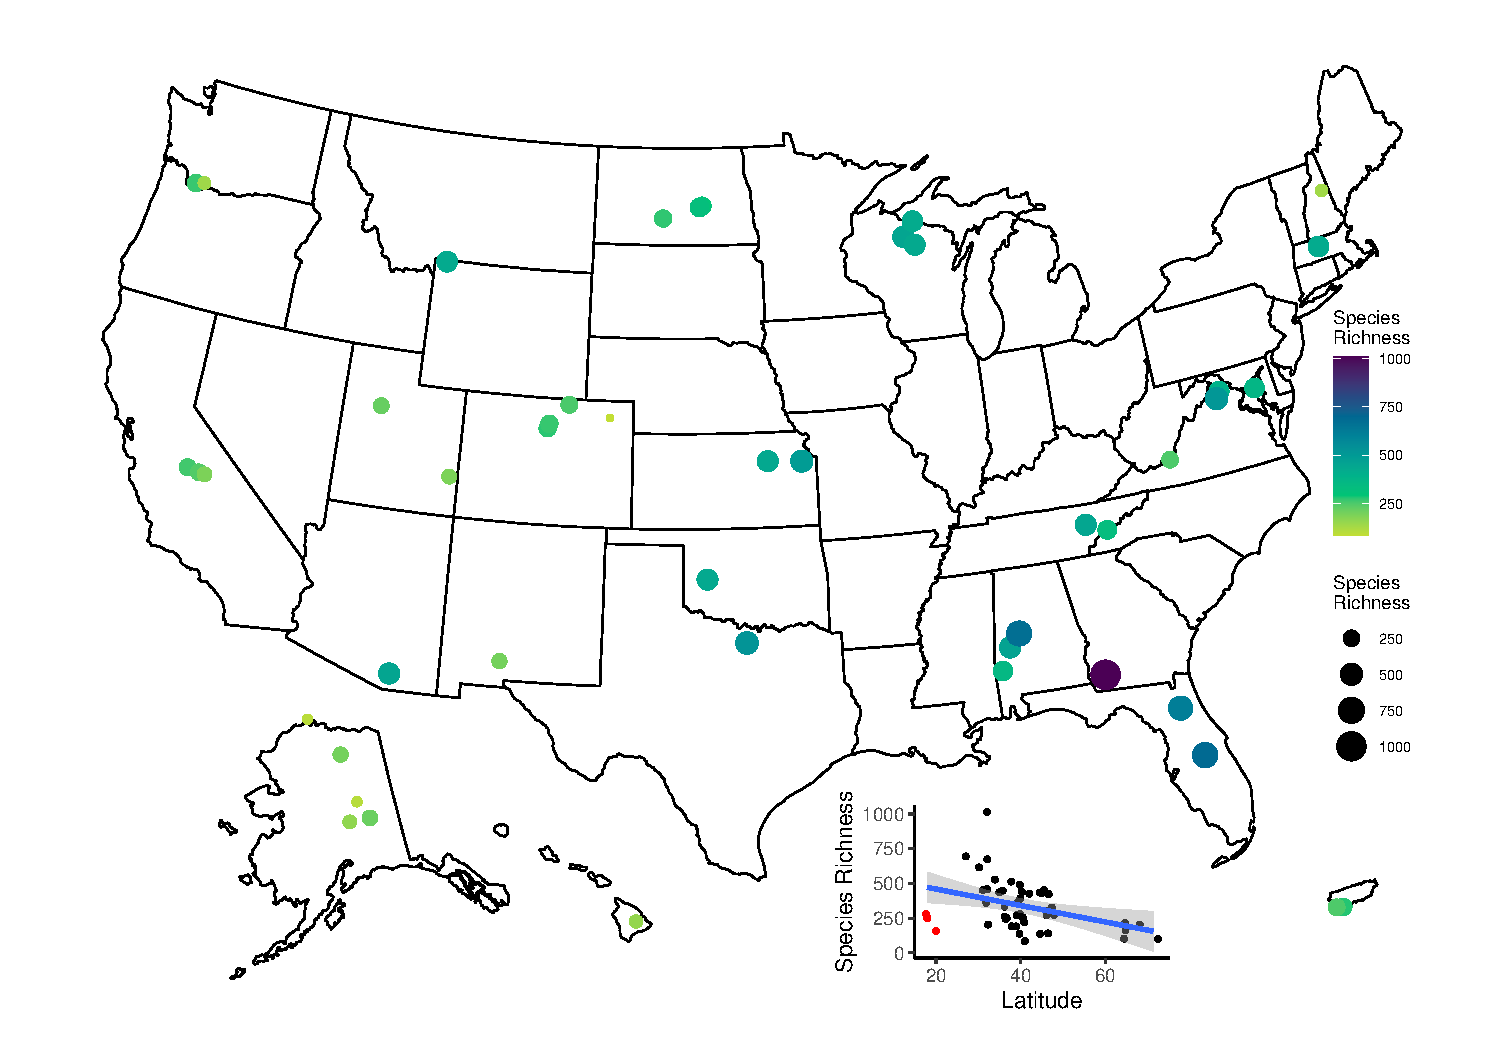
\includegraphics[width=0.95\linewidth]{/Users/dli/Github/neonDivData/manuscript/figures/p_plant} 

}

\caption{Plant species richness mapped across NEON terrestrial sites. The inset scatterplot shows latitude on the x-axis and species richness on the y-axis, with red points representing sites in Puerto Rico and Hawaii.}\label{fig:Fig2Map}
\end{figure}

In addition to allowing for quick exploration of macroecological patterns of richness at NEON sites, the data packages presented in this paper enable investigation of effects of taxonomic resolution on diversity indices since taxonomic information is preserved for observations under family level for all groups. The degree of taxonomic resolution varies for NEON taxa depending on the diversity of the group and the level of taxonomic expertise needed to identify an organism to the species level, with more diverse groups presenting a greater challenge. Beetles are one of the most diverse groups of organisms on Earth and wide-ranging geographically, making them ideal bioindicators of environmental change (Rainio and Niemelä 2003). To illustrate how the use of the beetle data package presented in this paper enables NEON data users to easily explore the effects of taxonomic resolution on community-level taxonomic diversity metrics, we calculated Jost diversity indices (Jost 2006) for beetles at the Oak Ridge National Laboratory (ORNL) NEON site for data subsetted at the genus, species, and subspecies level. To quantify biodiversity, we used Jost indices, which are essentially Hill Numbers that vary in how abundance is weighted with a parameter \emph{q}. Higher values of \emph{q} give lower weights to low-abundance species, with \emph{q} = 0 being equivalent to species richness and \emph{q} = 1 representing the effective number of species given by the Shannon entropy. These indices are plotted as rarefaction curves, which assess the sampling efficacy. When rarefaction curves asymptote they suggest that additional sampling will not capture additional taxa. Statistical methods presented by Chao et al. (2014) provide estimates of sampling efficacy beyond the observed data (i.e., extrapolated values shown by dashed lines in Fig. \ref{fig:Fig3Curve}). For the ORNL beetle data, Jost indices calculated with higher values of \emph{q} (i.e., \emph{q} \textgreater{} 0) indicated sampling has reached an asymptote in terms of capturing diversity regardless of taxonomic resolution (i.e., genus, species, subspecies). However, rarefaction curves for \emph{q} = 0, which is equivalent to species richness do not asymptote, even with extrapolation. These plots suggest that if a researcher is interested in low abundance, rare species, then the NEON beetle data stream at ORNL may need to mature with additional sample collections over time before confident inferences may be made, especially below the taxonomic resolution of genus.



\begin{figure}

{\centering 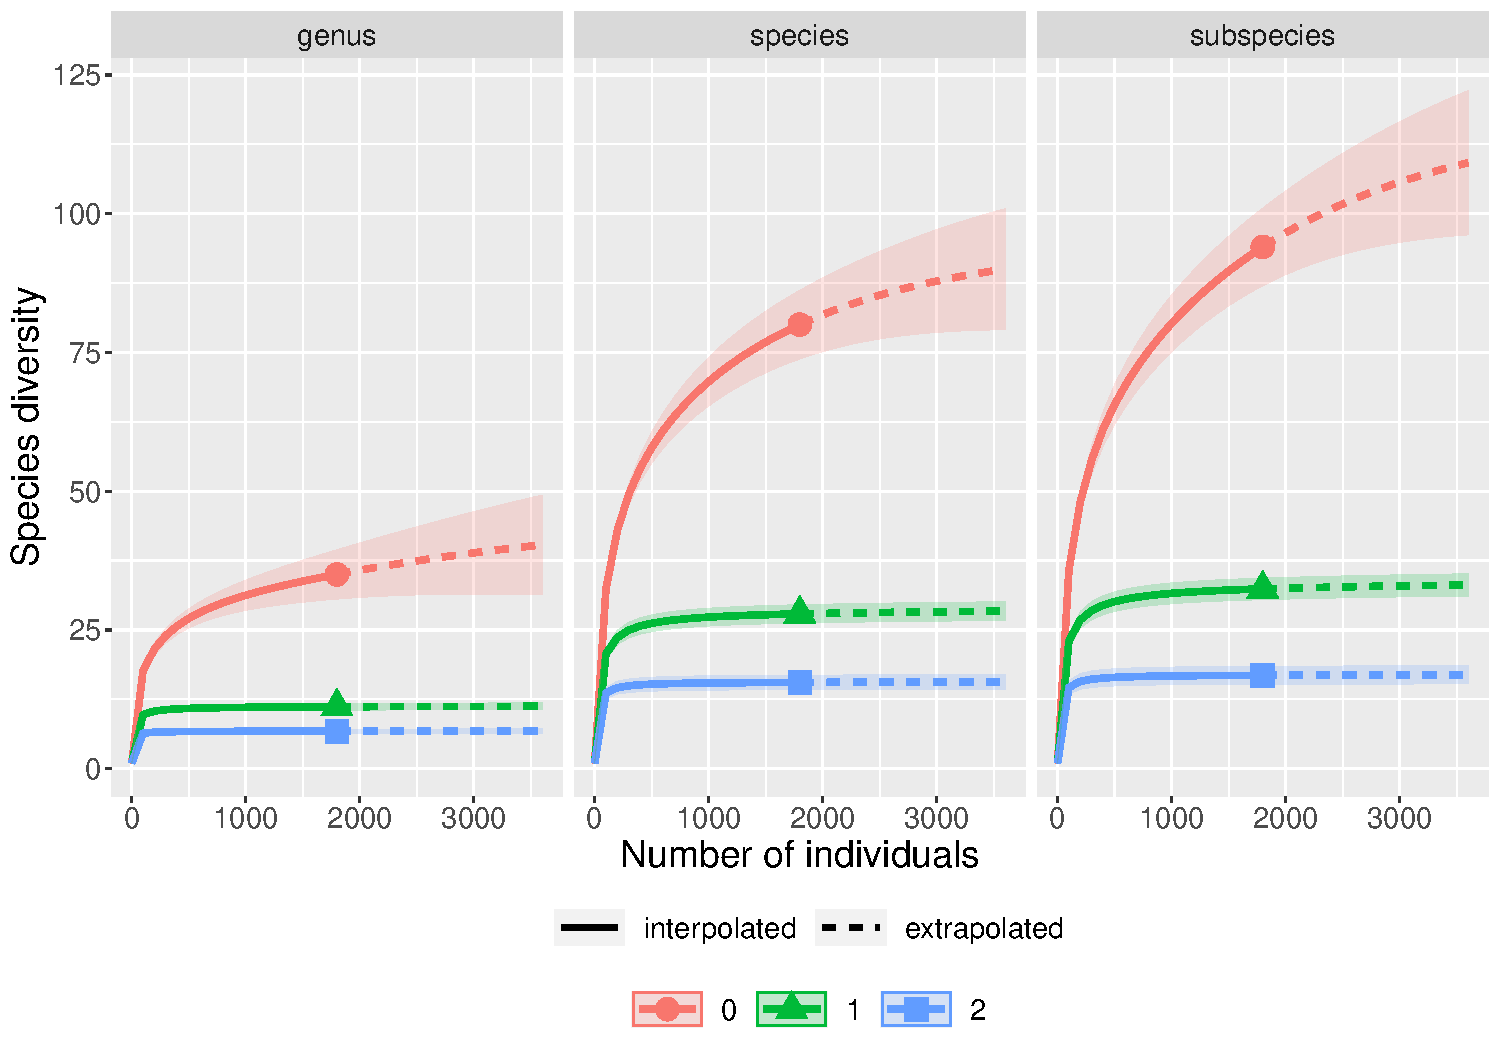
\includegraphics[width=0.95\linewidth]{/Users/dli/Github/neonDivData/manuscript/figures/beetle_rarefaction} 

}

\caption{Rarefaction of beetle abundance data from collections made at the Oak Ridge National Laboratory (ORNL) National Ecological Observatory Network (NEON) site from 2014-2020 generated using the beetle data package presented in this paper and the iNEXT package in R (Hsieh et al. 2016) based on different levels of taxonomic resolution (i.e., genus, species, subspecies). Different colors indicate Jost Indices with differing values of q (Jost 2006).}\label{fig:Fig3Curve}
\end{figure}

\hypertarget{discussion-or-how-to-maintain-and-update-standardized-neon-organismal-data}{%
\section{Discussion (or how to maintain and update standardized NEON organismal data)}\label{discussion-or-how-to-maintain-and-update-standardized-neon-organismal-data}}

NEON organismal data hold enormous potential to understand biodiversity change across space and time (Balch et al. 2019, Jones et al. 2021). Multiple biodiversity research and education programs have used NEON data even before NEON became fully operational in May 2019 (e.g., Farrell and Carey 2018, Read et al. 2018). With the expected long-term investment to maintain NEON over the next 30 years, NEON organismal data will be an invaluable tool for understanding and tracking biodiversity change. NEON data are unique relative to data collected by other similar networks (e.g., LTER, CZO) because observation collection protocols are standardized across sites, enabling researchers to address macroscale questions in environmental science without having to synthesize disparate data sets that differ in collection methods (Jones et al. 2021). The data package presented in this paper holds great potential in making NEON data easier to use and more comparable across studies. Whereas the data collection protocols implemented by NEON staff are standardized, the decisions NEON data users make in wrangling their data after downloading NEON's open data will not necessarily be similar unless the user community adopts a community data standard, such as the ecocomDP data model. Adopting such a data model early on in the life of the observatory will ensure that results of studies using NEON data will be comparable and thus easier to synthesize. By providing a standardized and easy-to-use data package of NEON organismal data, our effort here will significantly lower the barriers to use the NEON organismal data for biodiversity research by many current and future researchers and will ensure that studies using NEON organismal data are comparable.

There are some important notes about the data package we provided. First, our processes assume that NEON ensured correct identifications of species. However, since records may be identified to any level of taxonomic resolution, and IDs above the genus level may not be useful for most biodiversity projects, we removed records with such IDs for groups that are relatively easy to identify (i.e., fish, plant, small mammals) or have very few taxon IDs that are above genus level (i.e., mosquito). However, for groups that are hard to identify (i.e., algae, beetle, bird, macroinvertebrate, tick, and tick pathogen), we decided to keep all records regardless of their taxon IDs level. Such information can be useful if we are interested in questions such as species-to-genus ratio or species rarefaction curves at different taxonomic levels (e.g., Fig. \ref{fig:Fig3Curve}). Users thus need to carefully consider which level of taxon IDs they need to address their research questions. Another note regarding species names is the term `sp.' vs `spp.' across NEON organismal data collections; the term `sp.' refers to a single morphospecies whereas the term `spp.' refers to more than one morphospecies. This is an important point to consider for community ecology or biodiversity analyses because it may add uncertainty into estimates of biodiversity metrics such as species richness. Second, we standardized species abundance measurements to make them comparable across different sampling events within each taxonomic group (Table \ref{tab:dataMapping}). Such standardization is critical to study and compare biodiversity. And finally, there are other organismal groups (Aquatic Microbes and Aquatic Plants; soil microbes are covered in Qin et al.~in prep) not included in this study given the complexity of the data.

All code for the Data Wrangling Decisions are available within the R package \texttt{ecocomDP} (\url{https://github.com/EDIorg/ecocomDP}). Users can modify the code if they need to make different decisions during the data wrangling process and update our workflows in our code by submitting a pull request to our Github repository. If researchers wish to generate their own derived organismal data sets from NEON data with slightly different decisions than the ones outlined in this paper, we recommend that they use the ecocomDP framework, contribute their workflow to the ecocomDP R package, upload the data to the EDI repository, and cite their data with the discoverable DOI given to them by EDI. Note that the ecocomDP data model was intended for community ecology analyses and may not be well suited for population-level analyses.

Because \texttt{ecocomDP} is an R package to access and format datasets following the ecocomDP format, we developed an R data package \texttt{neonDivData} to host and distribute the standardized NEON organismal data derived from \texttt{ecocomDP}. A separate dedicated data package has several advantages. First, it is easier and ready to use and saves time for users to run the code in \texttt{ecocomDP} to download and standardize NEON data products. Second, it is also easy to update the data package when new raw data products are uploaded by NEON to their data portal; and the updating process does not require any change in the \texttt{ecocomDP} package. This is ideal because \texttt{ecocomDP} provides harmonized data from other sources besides NEON. Third, the \href{(https://github.com/daijiang/neonDivData)}{Github repository page of \texttt{neonDivData}} can serve as a discussion forum for researchers regarding the NEON data products without competing for attention in the \texttt{ecocomDP} Github repository page. By opening issues on the Github repository, users can discuss and contribute to improve our workflow of standardizing NEON data products. Users can also discuss whether there are other data models that the NEON user community should adopt at the inception of the observatory. As the observatory moves forward, this is an important discussion for the NEON user community and NEON technical working groups to promote synthesis of NEON data with data from other efforts (e.g., LTER, CZO, Ameriflux, the International LTER, National Phenology Network, Long Term Agricultural Research Network). Note that the standardized datasets that are stable (defined by NEON as stable release) were archived at EDI and some of the above advantages also apply to the data repository at EDI.

The derived data products presented here collectively represent hundreds of hours of work by members of our team - a group that met at the NEON Science Summit in 2019 in Boulder, Colorado and consists of researchers and NEON science staff. Just as it is helpful when working with a dataset to either have collected the data or be in close correspondence with the person who collected the data, final processing decisions were greatly informed by conversations with NEON science staff and the NEON user community. Future opportunities that encourage collaborations between NEON science staff and the NEON user community will be essential to achieve the full potential of the observatory data.

\hypertarget{conclusion}{%
\section{Conclusion}\label{conclusion}}

Macrosystems ecology (sensu Heffernan et al. 2014) is at the start of an exciting new chapter with the decades long awaited buildout of NEON completed and standardized data streams from all sites in the observatory becoming publicly available online. As the research community embarks on discovering new scientific insights from NEON data, it is important that we make our analyses and all derived data as reproducible as possible to ensure that connections across studies are possible. Harmonized data sets will help in this endeavour because they naturally promote the collection of provenance as data are collated into derived products (O'Brien et al.~In review, Reichman et al. 2011). Harmonized data also make synthesis easier because efforts to clean and format data leading up to analyses do not have to be repeatedly performed by individual researchers (O' Brien et al.~In review). The data standardizing processes and derived data package presented here illustrate a potential path forward in achieving a reproducible framework for data derived from NEON organismal data for ecological analyses. This derived data package also highlights the value of collaboration between the NEON user community and NEON staff for advancing NEON-enabled science.

\hypertarget{acknowledgement}{%
\section{Acknowledgement}\label{acknowledgement}}

This work is a result of participating in the first NEON Science Summit in 2019 and an internship program through the St.~Edward's Institute for Interdisciplinary Science (i4) funded through a National Science Foundation award under Grant No.~1832282. The authors acknowledge support from the NSF Award \#1906144 to attend the 2019 NEON Science Summit. Additionally, the authors acknowledge support from the NSF DEB 1926568 to S.R., NSF DEB 1926567 to P.L.Z., NSF DEB 1926598 to M.A.J, and NSF DEB 1926341 to J.M.L.. Comments from NEON staff (Katie LeVan, Dylan Mpnahan, Sata Paull, Dave Barnett, Sam Simkin), Margaret O'Brien and Tad Dallas greatly improved this work. The National Ecological Observatory Network is a program sponsored by the National Science Foundation and operated under cooperative agreement by Battelle Memorial Institute. This material is based in part upon work supported by the National Science Foundation through the NEON Program.

\hypertarget{reference}{%
\section*{Reference}\label{reference}}
\addcontentsline{toc}{section}{Reference}

\hypertarget{refs}{}
\begin{CSLReferences}{1}{0}
\leavevmode\hypertarget{ref-baker1997environmental}{}%
Baker, J. R., D. V. Peck, and D. W. Sutton. 1997. Environmental monitoring and assessment program surface waters: Field operations manual for lakes. US Environmental Protection Agency, Washington.

\leavevmode\hypertarget{ref-balch2019neon}{}%
Balch, J. K., R. Nagy, and B. S. Halpern. 2019. NEON is seeding the next revolution in ecology. Frontiers in Ecology and the Environment 18.

\leavevmode\hypertarget{ref-Barnett2019}{}%
Barnett, D. 2019. TOS protocol and procedure: DIV - plant diversity sampling. NEON.DOC.014042vK. NEON (National Ecological Observatory Network).

\leavevmode\hypertarget{ref-barnett2019plant}{}%
Barnett, D. T., P. B. Adler, B. R. Chemel, P. A. Duffy, B. J. Enquist, J. B. Grace, S. Harrison, R. K. Peet, D. S. Schimel, T. J. Stohlgren, and others. 2019. The plant diversity sampling design for the national ecological observatory network. Ecosphere 10:e02603.

\leavevmode\hypertarget{ref-bechtold2005enhanced}{}%
Bechtold, W. A., and P. L. Patterson. 2005. The enhanced forest inventory and analysis program--national sampling design and estimation procedures. USDA Forest Service, Southern Research Station.

\leavevmode\hypertarget{ref-beck2014spatial}{}%
Beck, J., M. Böller, A. Erhardt, and W. Schwanghart. 2014. Spatial bias in the GBIF database and its effect on modeling species' geographic distributions. Ecological Informatics 19:10--15.

\leavevmode\hypertarget{ref-blowes2019geography}{}%
Blowes, S. A., S. R. Supp, L. H. Antão, A. Bates, H. Bruelheide, J. M. Chase, F. Moyes, A. Magurran, B. McGill, I. H. Myers-Smith, and others. 2019. The geography of biodiversity change in marine and terrestrial assemblages. Science 366:339--345.

\leavevmode\hypertarget{ref-brown2004toward}{}%
Brown, J. H., J. F. Gillooly, A. P. Allen, V. M. Savage, and G. B. West. 2004. Toward a metabolic theory of ecology. Ecology 85:1771--1789.

\leavevmode\hypertarget{ref-Cawley2016}{}%
Cawley, K. M., S. Parker, R. Utz, K. Goodman, C. Scott, M. Fitzgerald, J. Vance, B. Jensen, C. Bohall, and T. Baldwin. 2016. NEON aquatic sampling strategy. NEON.DOC.001152vA. NEON (National Ecological Observatory Network).

\leavevmode\hypertarget{ref-chao2014rarefaction}{}%
Chao, A., N. J. Gotelli, T. Hsieh, E. L. Sander, K. Ma, R. K. Colwell, and A. M. Ellison. 2014. Rarefaction and extrapolation with hill numbers: A framework for sampling and estimation in species diversity studies. Ecological monographs 84:45--67.

\leavevmode\hypertarget{ref-Chesney2021}{}%
Chesney, T., S. Parker, and C. Scott. 2021. NEON user guide to aquatic macroinvertebrate collection (DP1.20120.001). Revision b. NEON (National Ecological Observatory Network).

\leavevmode\hypertarget{ref-curtis1959vegetation}{}%
Curtis, J. T. 1959. The vegetation of wisconsin: An ordination of plant communities. University of Wisconsin Pres.

\leavevmode\hypertarget{ref-egli2020taxonomic}{}%
Egli, L., K. E. LeVan, and T. T. Work. 2020. Taxonomic error rates affect interpretations of a national-scale ground beetle monitoring program at national ecological observatory network. Ecosphere 11:e03035.

\leavevmode\hypertarget{ref-Elmendorf2018}{}%
Elmendorf, S., and H. Brownlee. 2018. NEON algorithm theoretical basis document (ATBD): OS general transitions. NEON.DOC.004825vA. NEON (National Ecological Observatory Network).

\leavevmode\hypertarget{ref-farley2018situating}{}%
Farley, S. S., A. Dawson, S. J. Goring, and J. W. Williams. 2018. Situating ecology as a big-data science: Current advances, challenges, and solutions. BioScience 68:563--576.

\leavevmode\hypertarget{ref-farrell2018power}{}%
Farrell, K. J., and C. C. Carey. 2018. Power, pitfalls, and potential for integrating computational literacy into undergraduate ecology courses. Ecology and evolution 8:7744--7751.

\leavevmode\hypertarget{ref-fischer1960latitudinal}{}%
Fischer, A. G. 1960. Latitudinal variations in organic diversity. Evolution 14:64--81.

\leavevmode\hypertarget{ref-g2019remote}{}%
G Pricope, N., K. L Mapes, and K. D Woodward. 2019. Remote sensing of human--environment interactions in global change research: A review of advances, challenges and future directions. Remote Sensing 11:2783.

\leavevmode\hypertarget{ref-geldmann2016determines}{}%
Geldmann, J., J. Heilmann-Clausen, T. E. Holm, I. Levinsky, B. Markussen, K. Olsen, C. Rahbek, and A. P. Tøttrup. 2016. What determines spatial bias in citizen science? Exploring four recording schemes with different proficiency requirements. Diversity and Distributions 22:1139--1149.

\leavevmode\hypertarget{ref-gurevitch1999statistical}{}%
Gurevitch, J., and L. V. Hedges. 1999. Statistical issues in ecological meta-analyses. Ecology 80:1142--1149.

\leavevmode\hypertarget{ref-hampton2013big}{}%
Hampton, S. E., C. A. Strasser, J. J. Tewksbury, W. K. Gram, A. E. Budden, A. L. Batcheller, C. S. Duke, and J. H. Porter. 2013. Big data and the future of ecology. Frontiers in Ecology and the Environment 11:156--162.

\leavevmode\hypertarget{ref-harte2011maximum}{}%
Harte, J. 2011. Maximum entropy and ecology: A theory of abundance, distribution, and energetics. OUP Oxford.

\leavevmode\hypertarget{ref-heffernan2014macrosystems}{}%
Heffernan, J. B., P. A. Soranno, M. J. Angilletta Jr, L. B. Buckley, D. S. Gruner, T. H. Keitt, J. R. Kellner, J. S. Kominoski, A. V. Rocha, J. Xiao, and others. 2014. Macrosystems ecology: Understanding ecological patterns and processes at continental scales. Frontiers in Ecology and the Environment 12:5--14.

\leavevmode\hypertarget{ref-hillebrand2004generality}{}%
Hillebrand, H. 2004. On the generality of the latitudinal diversity gradient. The American Naturalist 163:192--211.

\leavevmode\hypertarget{ref-hoekman2017design}{}%
Hoekman, D., K. E. LeVan, C. Gibson, G. E. Ball, R. A. Browne, R. L. Davidson, T. L. Erwin, C. B. Knisley, J. R. LaBonte, J. Lundgren, and others. 2017. Design for ground beetle abundance and diversity sampling within the national ecological observatory network. Ecosphere 8:e01744.

\leavevmode\hypertarget{ref-hsieh2016inext}{}%
Hsieh, T., K. Ma, and A. Chao. 2016. iNEXT: An r package for rarefaction and extrapolation of species diversity (h ill numbers). Methods in Ecology and Evolution 7:1451--1456.

\leavevmode\hypertarget{ref-hubbell2001unified}{}%
Hubbell, S. P. 2001. The unified neutral theory of biodiversity and biogeography (MPB-32). Princeton University Press.

\leavevmode\hypertarget{ref-hutchinson1959homage}{}%
Hutchinson, G. E. 1959. Homage to santa rosalia or why are there so many kinds of animals? The American Naturalist 93:145--159.

\leavevmode\hypertarget{ref-Jensen2019a}{}%
Jensen, B., S. Parker, and J. R. Fischer. 2019a. AOS protocol and procedure: Fish sampling in wadeable streams. NEON.DOC.001295vF. NEON (National Ecological Observatory Network).

\leavevmode\hypertarget{ref-Jensen2019b}{}%
Jensen, B., S. Parker, and J. R. Fischer. 2019b. AOS protocol and procedure: Fish sampling in lakes. NEON.DOC.001296vF. NEON (National Ecological Observatory Network).

\leavevmode\hypertarget{ref-jones2021synergies}{}%
Jones, J., P. Groffman, J. Blair, F. Davis, H. Dugan, E. Euskirchen, S. Frey, T. Harms, E. Hinckley, M. Kosmala, and others. 2021. Synergies among environmental science research and monitoringnetworks: A research agenda. Earth's Future:e2020EF001631.

\leavevmode\hypertarget{ref-jost2006entropy}{}%
Jost, L. 2006. Entropy and diversity. Oikos 113:363--375.

\leavevmode\hypertarget{ref-keller2008continental}{}%
Keller, M., D. S. Schimel, W. W. Hargrove, and F. M. Hoffman. 2008. A continental strategy for the national ecological observatory network. The Ecological Society of America: 282-284.

\leavevmode\hypertarget{ref-koricheva2014uses}{}%
Koricheva, J., and J. Gurevitch. 2014. Uses and misuses of meta-analysis in plant ecology. Journal of Ecology 102:828--844.

\leavevmode\hypertarget{ref-LeVan2020}{}%
LeVan, K. 2020a. NEON user guide to ground beetles sampled from pitfall traps (DP1.10022.001).version c. NEON (National Ecological Observatory Network).

\leavevmode\hypertarget{ref-LeVan2020b}{}%
LeVan, K. 2020b. NEON user guide to mosquitoes sampled from CO2 traps (DP1.10043.001) and mosquito-borne pathogen satatus (DP1.10041.001).version c. NEON (National Ecological Observatory Network).

\leavevmode\hypertarget{ref-LeVan2019b}{}%
LeVan, K., S. Paull, K. Tsao, D. Hoekman, and Y. Springer. 2019a. TOS protocol and procedure: MOS - mosquito sampling. NEON.DOC.014049vL. NEON (National Ecological Observatory Network).

\leavevmode\hypertarget{ref-LeVan2019}{}%
LeVan, K., N. Robinson, D. Hoekman, and K. Blevins. 2019b. TOS protocol and procedure: Ground beetle sampling. NEON.DOC.014041vJ. NEON (National Ecological Observatory Network).

\leavevmode\hypertarget{ref-LeVan2019c}{}%
LeVan, K., K. Thibault, K. Tsao, and Y. Springer. 2019c. TOS protocol and procedure: Tick and tick-borne pathogen sampling. NEON.DOC.014045vK. NEON (National Ecological Observatory Network).

\leavevmode\hypertarget{ref-li2020changes}{}%
Li, D., J. D. Olden, J. L. Lockwood, S. Record, M. L. McKinney, and B. Baiser. 2020. Changes in taxonomic and phylogenetic diversity in the anthropocene. Proceedings of the Royal Society B 287:20200777.

\leavevmode\hypertarget{ref-linnaeus1758systema}{}%
Linnaeus, C. 1758. Systema naturae. Stockholm Laurentii Salvii.

\leavevmode\hypertarget{ref-macarthur1967theory}{}%
MacArthur, R. H., and E. O. Wilson. 1967. The theory of island biogeography. Princeton university press.

\leavevmode\hypertarget{ref-martin2012mapping}{}%
Martin, L. J., B. Blossey, and E. Ellis. 2012. Mapping where ecologists work: Biases in the global distribution of terrestrial ecological observations. Frontiers in Ecology and the Environment 10:195--201.

\leavevmode\hypertarget{ref-midgley2005global}{}%
Midgley, G. F., and W. Thuiller. 2005. Global environmental change and the uncertain fate of biodiversity. The New Phytologist 167:638--641.

\leavevmode\hypertarget{ref-Monahan2020}{}%
Monahan, D., B. Jensen, S. Parker, and C. Scott. 2020. NEON user guide to fish electrofishing, gill netting, and fyke netting counts (DP1.20107.001). Revision b. NEON (National Ecological Observatory Network).

\leavevmode\hypertarget{ref-moulton2002revised}{}%
Moulton II, S. R., J. G. Kennen, R. M. Goldstein, and J. A. Hambrook. 2002. Revised protocols for sampling algal, invertebrate, and fish communities as part of the national water-quality assessment program. Geological Survey (US).

\leavevmode\hypertarget{ref-nakagawa2012methodological}{}%
Nakagawa, S., and E. S. Santos. 2012. Methodological issues and advances in biological meta-analysis. Evolutionary Ecology 26:1253--1274.

\leavevmode\hypertarget{ref-palumbo2017building}{}%
Palumbo, I., R. A. Rose, R. M. Headley, J. Nackoney, A. Vodacek, and M. Wegmann. 2017. Building capacity in remote sensing for conservation: Present and future challenges. Remote Sensing in Ecology and Conservation 3:21--29.

\leavevmode\hypertarget{ref-Parker2019}{}%
Parker, S. 2019. AOS protocol and procedure: INV - aquatic macroinvertebrate sampling. NEON.DOC.003046vE. NEON (National Ecological Observatory Network).

\leavevmode\hypertarget{ref-Parker2020}{}%
Parker, S. 2020. AOS protocol and procedure: ALG - periphyton and phytoplankton sampling. NEON.DOC.003045vE. NEON (National Ecological Observatory Network).

\leavevmode\hypertarget{ref-ParkerRoehm2019}{}%
Parker, S., and C. Roehm. 2019. AOS protocol and procedure: ZOO - zooplankton sampling in lakes. NEON.DOC.001194. NEON (National Ecological Observatory Network).

\leavevmode\hypertarget{ref-ParkerScott2020}{}%
Parker, S., and C. Scott. 2020. NEON user guide to aquatic zooplankton collection (DP1.20219.001). Revision b. NEON (National Ecological Observatory Network).

\leavevmode\hypertarget{ref-ParkerVance2020}{}%
Parker, S., and T. Vance. 2020. NEON user guide to periphyton and phytoplankton collection (DP1.20166.001). Revision c. NEON (National Ecological Observatory Network).

\leavevmode\hypertarget{ref-pavlacky2017statistically}{}%
Pavlacky Jr, D. C., P. M. Lukacs, J. A. Blakesley, R. C. Skorkowsky, D. S. Klute, B. A. Hahn, V. J. Dreitz, T. L. George, and D. J. Hanni. 2017. A statistically rigorous sampling design to integrate avian monitoring and management within bird conservation regions. PloS one 12:e0185924.

\leavevmode\hypertarget{ref-peck2006environmental}{}%
Peck, D. V., Herlihy, A. T., Hill, B. H., Hughes, R. M., Kaufmann, P. R., Klemm, D. J., Lazorchak, J. M., McCormick, F. H., Peterson, S. A., Ringold, P. L., Magee, T., and M. R. and Cappaert. 2006. Environmental monitoring and assessment program --- surface waters: Western pilot study field operations manual for wadeable streams. US Environmental Protection Agency, Washington.

\leavevmode\hypertarget{ref-pritt2017proposal}{}%
Pritt, B. S., M. E. Allerdice, L. M. Sloan, C. D. Paddock, U. G. Munderloh, Y. Rikihisa, T. Tajima, S. M. Paskewitz, D. F. Neitzel, D. K. H. Johnson, and others. 2017. Proposal to reclassify ehrlichia muris as ehrlichia muris subsp. Muris subsp. Nov. And description of ehrlichia muris subsp. Eauclairensis subsp. Nov., A newly recognized tick-borne pathogen of humans. International journal of systematic and evolutionary microbiology 67:2121.

\leavevmode\hypertarget{ref-rainio2003ground}{}%
Rainio, J., and J. Niemelä. 2003. Ground beetles (coleoptera: Carabidae) as bioindicators. Biodiversity \& Conservation 12:487--506.

\leavevmode\hypertarget{ref-ralph1993handbook}{}%
Ralph, C. J. 1993. Handbook of field methods for monitoring landbirds. Pacific Southwest Research Station.

\leavevmode\hypertarget{ref-read2018among}{}%
Read, Q. D., J. M. Grady, P. L. Zarnetske, S. Record, B. Baiser, J. Belmaker, M.-N. Tuanmu, A. Strecker, L. Beaudrot, and K. M. Thibault. 2018. Among-species overlap in rodent body size distributions predicts species richness along a temperature gradient. Ecography 41:1718--1727.

\leavevmode\hypertarget{ref-record2020novel}{}%
Record, S., N. M. Voelker, P. L. Zarnetske, N. I. Wisnoski, J. D. Tonkin, C. Swan, L. Marazzi, N. Lany, T. Lamy, A. Compagnoni, and others. 2020. Novel insights to be gained from applying metacommunity theory to long-term, spatially replicated biodiversity data. Frontiers in Ecology and Evolution 8:479.

\leavevmode\hypertarget{ref-reichman2011challenges}{}%
Reichman, O. J., M. B. Jones, and M. P. Schildhauer. 2011. Challenges and opportunities of open data in ecology. Science 331:703--705.

\leavevmode\hypertarget{ref-rudenko2011updates}{}%
Rudenko, N., M. Golovchenko, L. Grubhoffer, and J. H. Oliver Jr. 2011. Updates on borrelia burgdorferi sensu lato complex with respect to public health. Ticks and tick-borne diseases 2:123--128.

\leavevmode\hypertarget{ref-sauer2017first}{}%
Sauer, J. R., K. L. Pardieck, D. J. Ziolkowski Jr, A. C. Smith, M.-A. R. Hudson, V. Rodriguez, H. Berlanga, D. K. Niven, and W. A. Link. 2017. The first 50 years of the north american breeding bird survey. The Condor: Ornithological Applications 119:576--593.

\leavevmode\hypertarget{ref-Stanish2020}{}%
Stanish, L., S. Weintraub, E.-L. S. Hinckley, and J. Parnell. 2020. TOS protocol and procedure: SLS - soil biogeochemical and microbial sampling. NEON.DOC.014048vN. NEON (National Ecological Observatory Network).

\leavevmode\hypertarget{ref-thibault2018TOS}{}%
Thibault, K. 2018. TOS protocol and procedure: Breeding landbird abundance and diversity. NEON.DOC.014041vJ. NEON (National Ecological Observatory Network).

\leavevmode\hypertarget{ref-thibault2019TOS}{}%
Thibault, K., K. Tsao, Y. Springer, and L. Knapp. 2019. TOS protocol and procedure: Small mammal sampling. NEON.DOC.000481vL. NEON (National Ecological Observatory Network).

\leavevmode\hypertarget{ref-thorpe2016introduction}{}%
Thorpe, A. S., D. T. Barnett, S. C. Elmendorf, E.-L. S. Hinckley, D. Hoekman, K. D. Jones, K. E. LeVan, C. L. Meier, L. F. Stanish, and K. M. Thibault. 2016. Introduction to the sampling designs of the n ational e cological o bservatory n etwork t errestrial o bservation s ystem. Ecosphere 7:e01627.

\leavevmode\hypertarget{ref-vellend2013global}{}%
Vellend, M., L. Baeten, I. H. Myers-Smith, S. C. Elmendorf, R. Beauséjour, C. D. Brown, P. De Frenne, K. Verheyen, and S. Wipf. 2013. Global meta-analysis reveals no net change in local-scale plant biodiversity over time. Proceedings of the National Academy of Sciences 110:19456--19459.

\leavevmode\hypertarget{ref-welti2021meta}{}%
Welti, E., A. Joern, A. M. Ellison, D. Lightfoot, S. Record, N. Rodenhouse, E. Stanley, and M. Kaspari. 2021. Meta-analyses of insect temporal trends must account for the complex sampling histories inherent to many long-term monitoring efforts. Nature Ecology and Evolution.

\leavevmode\hypertarget{ref-wilkinson2016fair}{}%
Wilkinson, M. D., M. Dumontier, Ij. J. Aalbersberg, G. Appleton, M. Axton, A. Baak, N. Blomberg, J.-W. Boiten, L. B. da Silva Santos, P. E. Bourne, and others. 2016. The FAIR guiding principles for scientific data management and stewardship. Scientific data 3:1--9.

\leavevmode\hypertarget{ref-worm2018theory}{}%
Worm, B., and D. P. Tittensor. 2018. A theory of global biodiversity (MPB-60). Princeton University Press.

\end{CSLReferences}

\end{document}
